\documentclass[a4paper,12pt,leqno]{article}
\usepackage[utf8]{inputenc}
\usepackage[ngerman]{babel}

\usepackage{amsmath}
\usepackage{amsthm}
\usepackage{amsfonts}
\usepackage{amssymb}
\usepackage[left=3cm,right=2cm,top=2cm,bottom=1.5cm]{geometry}
\usepackage{parskip}
\usepackage{graphicx}
\usepackage{caption}
\usepackage{hyperref}
\usepackage{upgreek}
\usepackage{mathtools}
\usepackage{tikz}
\hypersetup{
    colorlinks,
    citecolor=black,
    filecolor=black,
    linkcolor=red,
    urlcolor=red
}

%%Code style
\usepackage{listings}
\usepackage{xcolor}
\definecolor{codegreen}{rgb}{0,0.6,0}
\definecolor{codegray}{rgb}{0.5,0.5,0.5}
\definecolor{codepurple}{rgb}{0.58,0,0.82}
\definecolor{backcolour}{rgb}{0.9,0.9,0.9}

\lstset{escapeinside={@}{@}}
\lstdefinestyle{mystyle}{
    backgroundcolor=\color{backcolour},   
    commentstyle=\color{codegreen},
    keywordstyle=\color{magenta},
    numberstyle=\tiny\color{codegray},
    stringstyle=\color{codepurple},
    basicstyle=\ttfamily\footnotesize,
    breakatwhitespace=false,         
    breaklines=true,                 
    captionpos=b,                    
    keepspaces=true,                 
    numbers=left,                    
    numbersep=5pt,                  
    showspaces=false,                
    showstringspaces=false,
    showtabs=false,                  
    tabsize=5
}

\lstset{style=mystyle}

\newcommand{\blue}[1]{\textcolor{blue}{#1}}
\newcommand{\orange}[1]{\textcolor{orange}{#1}}
\newcommand{\violet}[1]{\textcolor{violet}{#1}}
%%End code style

\title{Computer System Sicherheit\\Notizen WS20/21}
\author{Felix Marx}

\begin{document}
\maketitle

{
%%Lokales Einfärben des Inhaltverzeichisses
\hypersetup{linkcolor=black}
\tableofcontents
}
\newpage

\section{Begriffe}
Unterscheidung \blue{Betriebssicherheit (safety)} und \blue{Angriffssicherheit (security)}.\\
safety bezeichnet den Schutz vor inneren Fehlern, deren Eintrittswahrscheinlichkeit durch probabilistische Techniken ermittelt wird.\\
security den Schutz gegen aktive Angreifer.

\subsection{Security}

Trends und Herausforderungen:\\
\textbf{Mobilität}, der Übergang zu ''smart devices''
\begin{figure}[h!]
\centering
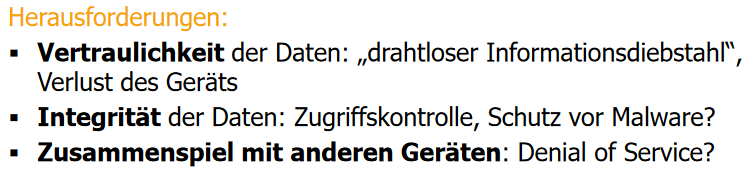
\includegraphics[scale=0.6]{Grafiken/Trend-Mobilitaet.png}
\caption{Herausforderungen bei der Mobilität}
\end{figure}

\textbf{Vernetzung}, der Übergang zu ''always on'' und Automatisierung von Systemen
\begin{figure}[h!]
\centering
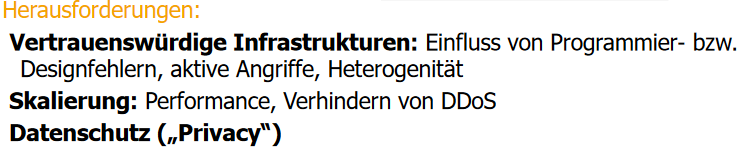
\includegraphics[scale=0.6]{Grafiken/Trend-Vernetzung.png}
\caption{Herausforderungen bei der Vernetzung}
\end{figure}

\textbf{Miniaturisierung}, Produktion kleinerer Chips mit Trend zu Einwegchips
\begin{figure}[h!]
\centering
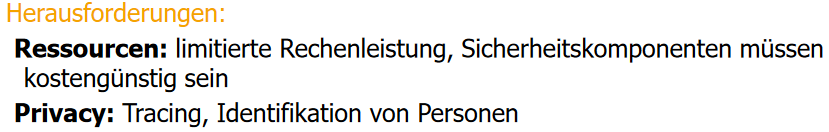
\includegraphics[scale=0.6]{Grafiken/Trend-Miniaturisierung.png}
\caption{Herausforderungen bei der Miniaturisierung}
\end{figure}\\

\blue{Social Engineering} bezeichnet das Erlangen von vertraulichen Daten durch psychologische Techniken\\
\blue{Man-in-the-middle} Angriffe, hier werden Nachrichten vor der gesicherten Kommunikation abgefangen.\\
Lösungen für \blue{Phishing} umfassen die Verifikation durch Transaktionsnummern (TANs) oder Hardwaretokens was allerding nicht die Integrität der Transaktion gewährleistet.\\
Schutzmechanismen:\\
\blue{Passive Authentication}: Sicherstellung der Authentizität durch Einsatz einer digitalen Signatur\\
\blue{Basic Access Control}: elektronische gespeicherte Daten werden erst übermittelt wenn das Lesegerät einen aufgedruckten maschinenlesbaren Code kennt.\\
\blue{Active Access Control}: Verhindert 1:1 Kopien indem ein geheimer Schlüssel in einem gesicherten Chip-Bereich gespeichert wird.\\
\blue{Extended Access Control}: Schutz von sensiblen Daten (Fingerabdruck, Iris, etc.) durch das Abgleichen von \href{https://en.wikipedia.org/wiki/Extended_Access_Control}{Zertifikaten} die nur eine kurze Zeit gültig sind.

\subsection{Safety}
Im Fehlerfall sollte ein System immer in den sicheren Zustand übergehen.\\
Zum Beispiel zeigt die Fahranweisung von Zügen nach oben, sodass es bei einem Schaden am Mechanismus in den Haltezustand nach unten fällt (Schwerkraft). Ein Watchdog (hier Schwerkraft) überwacht quasi das System auf Fehler und resettet es bei einem Fehler.

\section{Verlässliche Systeme}
Ein zuverlässiges System erfüllt seinen Zweck auch falls Fehler auftreten.
\begin{figure}
\centering
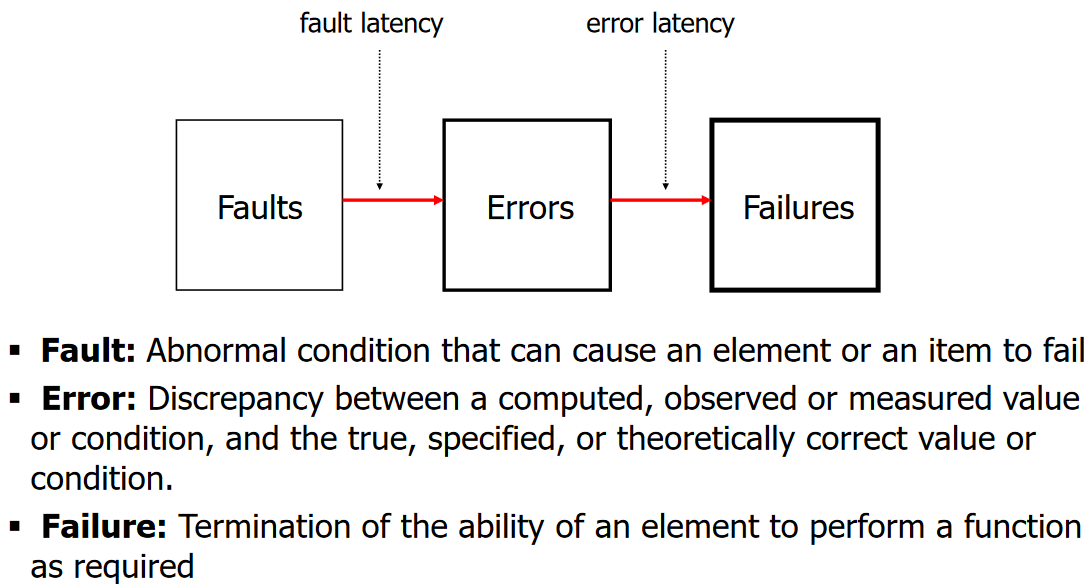
\includegraphics[scale=0.4]{Grafiken/AblaufZumVersagen.png}
\caption{Ablauf bis ein System versagt}
\label{Image:Versagensplan}
\end{figure}
Als Beispiel des \hyperref[Image:Versagensplan]{Ablaufes} lässt sich die Einwirkung von kosmischer Strahlung auf eine DRAM-Zelle (Fault) was zum Wechsel eines Wertes führt (Error), wodurch die Berechnung ein falsches Ergebnis liefert (Failure).\\
In der Zuverlässigkeit wird unterschieden nach:\\
\textbf{Availability}: Verfügbarkeit eines Systems gemessen in Prozent, d.h. 
$$\frac{\textrm{Total Up Time}}{\textrm{Total (Up + Down Time)}}=\frac{\textrm{MTTF}}{\textrm{MTTF + MTTR}}$$
\textbf{Reliability}: Zuverlässigkeit eines Systems, d.h. die Wahrscheinlichkeit dass ein System über einen gewissen Zeitraum korrekt funktioniert.\\
Wir bezeichnen mit \blue{MTTF} die Mean Time To Failure und mit \blue{MTTR} Mean Time To Recovery. Bei der Berechnung wird für die Up/Downtime nur die Zeiten im vereinbarten Betriebszeitraum gezählt!\\
Die Wahrscheinlichkeit, dass ein System bis zum Zeitpunkt $t$ fehlerhaft wird lässt sich mittels einer Verteilerfunktion $F$ und der Lebenszeit des Systems T berechnen:
$$F(t)=P(T\leq t)\textrm{, } R(t)=P(T>t)=1-F(t)$$
Die Funktion $R$ hingegen ermittelt die Wahrscheinlichkeit, dass ein System bis zum Zeitpunkt $t$ korrekt funktioniert.
Geht man davon aus, dass zukünftige Ausfälle unabhängig davon passieren, wann der letzte Ausfall war, lässt sich die Wahrscheinlichkeit mit einer Fehlerrate $\lambda$ so ausdrücken:\\
\begin{align*}
f(x) = &
\begin{cases} 
	\lambda e^{-\lambda x} & x\geq 0\\
	 0 & x < 0
\end{cases} \\
F(t) = & \int_{-\infty}^t f(x)dx = &
\begin{cases}
1 -e^{-\lambda t} & t \geq 0\\
0 & t < 0
\end{cases}\\
R(t) = & 1 -F(t) = & 
\begin{cases}
e^{-\lambda t} & t \geq 0\\
1 & t< 0
\end{cases}
\end{align*}
\begin{figure}[h!]
\centering
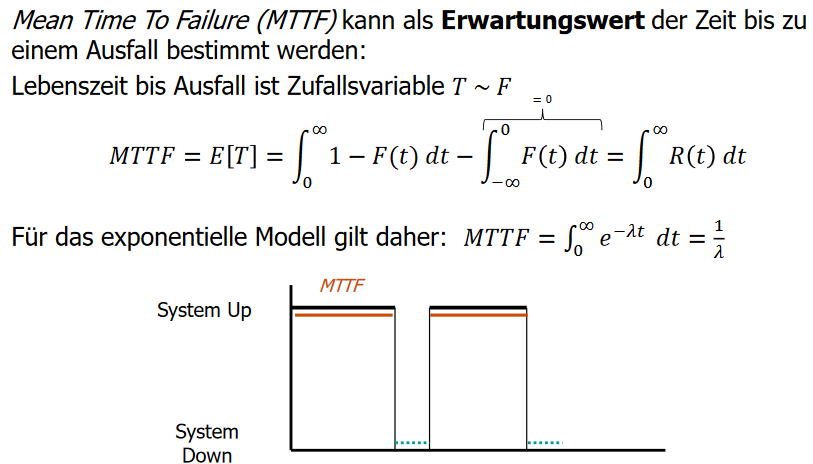
\includegraphics[scale=0.6]{Grafiken/MTTF-Model.png}
\caption{Berechnung MTTF mit dem exponentiellen Model}
\end{figure}\\
Bei in Reihe geschalteten Komponenten wird die Wahrscheinlichkeit dass das gesamte System korrekt funktioniert R durch $R_{ges}(t)=\prod^n_{i=1}R_i(t)$ im exponentiellen Modell wird dann für $\lambda = \lambda_{ges}=\sum_{i=1}^n\lambda_i$ verwendet.\\
Bei Parallelschaltung ist die Wahrscheinlichkeit dass das System korrekt funktioniert:
$$R_{ges}(t)=R_1(t)+R_2(t)-R_1(t)\cdot R_2(t), F_{ges}(t)=F_1(t)\cdot F_2(t)$$
Bei mehr als zwei Komponenten ist die allgemeine Formel:
$$R_{ges}(t)=1-\prod_{i=1}^n(1-R_i(t)), F_{ges}(t)=\prod_{i=1}^nF_i(t)$$

\subsection{Strategien zur Fehlervermeidung/toleranz}
\begin{itemize}
\item Fehlervermeidung (fault avoidance)
	\begin{itemize}
	\item Design des Systems stellt sicher, dass Fehler nicht auftreten
	\item Beispiel: Testen, Verifikation,...
	\end{itemize}
\item Wiederherstellung aus Fehlerzustand (fault recovery)
	\begin{itemize}
	\item Strategien, um ein System beim Auftreten eines Fehlers wieder in einen korrekten Systemzustand zu bringen
	\end{itemize}
\item Fehlertoleranz (fault tolerance)
	\begin{itemize}
	\item Wenn Fehler nicht vermieden werden können, dann soll das System Fehler tolerieren
	\item Beispiele: Redundanz, Safety, ...
	\end{itemize}
\end{itemize}
\textbf{Arten von Redundanzen:}
\begin{itemize}
\item Physikalische Redundanz (physical redundancy)
	\begin{itemize}
	\item Zusätzliche Ressourcen bzw. Komponenten
	\item Berechnungen werden auf mehreren Komponenten ausgeführt und verglichen
	\item Statische Redundanz
		\begin{itemize}
		\item $N$ Systeme laufen parallel
		\item $N-1$ Systeme laufen im  ''stand-by-mode''
		\item Bei einem Fehler wird im Betrieb umgeschaltet
		\item Dazu muss man den Fehler natürlich zuerst erkennen!
		\end{itemize}
	\item Dynamische Redundanz
		\begin{itemize}
		\item $N$ Systeme laufen parallel
		\item Ausfallsicherhere Komponente vergleicht die Resultate
		\item Mehrheitsentscheidung (zB. 2-out-of-3)
		\item Erkennt Fehler ''automatisch''
		\end{itemize}
	\end{itemize}
\item Zeitliche Redundanz (temporal redundancy)
	\begin{itemize}
	\item Berechnungen auf gleicher Hardware-Plattform wiederholen
	\end{itemize}
\item Redundanzen durch (Zusatz-)Information (information redundancy)
	\begin{itemize}
	\item Hinzufügen von zusätzlichen Daten (Checksummen, ...)
	\item Erlaubt Datenfelder bei Übertragung oder Speicherung zu erkennen
	\end{itemize}
\end{itemize}
Bei dynamischer Redundanz wird das Ergebnis parallel berechnet und dann per Mehrheitsentscheidung das korrekte ausgewählt. Problematisch falls im Vergleich ein Problem auftritt. Softwarefehler sind von der Hardware-Redundanz nicht abgedeckt.
Zusatzinformationen können die Integrität gesendeter Daten durch Checksummen sicherstellen, allerdings auch nur begrenzt.\\

Nachteile von Redundanzen sind:
\begin{itemize}
\item Schlechtere Performanz (bei temporaler Redundanz)
\item Synchronisation erforderlich
\item Hohe Kosten durch mehrfache Hardware bzw. mehrfache Implemenation (falls überhaupt möglich)
\item Benötigt Mechanismen zur Fehler-Erkennung, welche selbst wieder Fehleranfällig sein können
\end{itemize}

\section{Krypographie}
\begin{itemize}
\label{item:schutzziele}
\item Vertraulichkeit (Confidentiality)
	\begin{itemize}
	\item Schutz vor unbefugten Zugriff auf Informationen / Daten
	\end{itemize}
\item Integrität
	\begin{itemize}
	\item Schutz vor Veränderung von Informationen / Daten
	\end{itemize}
\item Verfügbarkeit (Availability)
	\begin{itemize}
	\item Daten oder Systeme sind verfügbar oder erreichbar
	\end{itemize}
\item Authentizität (Authenticity)
	\begin{itemize}
	\item Garantie dass die Daten auch aus der angegebenen Quelle stammen
	\end{itemize}
\item Nicht-Abstreitbarkeit (Non-Repudiation)
	\begin{itemize}
	\item Aktion ist nachprüfbar und kann nicht abgestritten werden
	\end{itemize}
\end{itemize}
\subsection{Begriffe}
\begin{itemize}
\item Klartext/Nachricht: eine zu verschlüsselnde Information
\item Klartextraum: Menge aller möglichen Klartexte
\item Chiffrat, Chiffretext: Verschlüsselte Nachricht
\item Chiffretextraum: Menge aller möglichen Chiffrate
\item Schlüssel: Ein Geheimnis, welches zur Ent-/Verschlüsselung benötigt wird
\item Schlüsselraum: Menge aller möglichen Schlüssel
\item Verschlüsselung: Umwandlung eines Klartext in ein Chiffrat
\item Entschlüsselung: Umwandlung eines Chiffrats in einen Klartext
\end{itemize}
\textbf{Kerckhoffs Prinzipien}
\begin{enumerate}
\item Das System muss praktisch, wenn nicht sogar mathematisch, unentschlüsselbar sein (''Unentschlüsselbarkeit'')
\item Es darf keine Geheimhaltung erfordern und darf ohne Schwierigkeiten  in die Hände des Feindes fallen (''Keine Geheimhaltung des Systems'')
\item Der Schlüssel muss ohne Hilfe geschriebener Notizen kommunizierbar und aufbewahrbar sein und er muss ausgewechselt oder modifiziert werden können nach Belieben der Kommunikationspartner (''Schlüssel ohne Aufschreiben'')
\item Es muss anwendbar sein auf die telegraphische Kommunikation
\item Es soll protabel sein und seine Funktion soll nicht die Zusammenkunft mehrerer Personen erfordern 
\item Schließlich ist es notwendig, angesichts der Umstände, unter denen es angewendet werden soll, dass das System einfach benutzbar ist und weder große gedankliche Anstrengung erfordert noch die Kenntnis einer langen Liste zu beachtender Regeln (''einfach benutzbar'')
\end{enumerate}
\subsection{Verschiebechiffre}
Die Ceasar-Chiffre ersetzt jeden Buchstaben des Klartextes durch den Buchstaben 3 Stellen weiter rechts, beim Entschlüsseln genau umgekehrt.\\
Die Verschiebechiffre ersetzt alle Buchstaben durch den Buchstaben welcher eine beliebige aber feste Anzahl an Stellen weiter rechts steht. Der Schlüssel ist die Anzahl an Verschiebungen, d.h. 0,1,2,...,25.

\subsection{Mathematische Grundlagen}
\label{def:Einwegfunktion}
Als \blue{Einwegfunktionen} bezeichnet man Funktionen deren Funktionswert $y = f(x)\in Y$ zu einem gegebenen $x$ in polynomieller Zeit berechenbar ist, aber ein Urbild $x\in f^{-1}[\{y\}]$ zu einem gegbenen $y$ nicht in Polynomialzeit bestimmbar ist. Die Existenz von Einwegfunktionen ist nicht bewiesen (P/NP).
\subsubsection{Teilbarkeitsregeln}
\begin{align}
a | a\\
a | b \wedge b |c \Rightarrow a|c\\
a|b\wedge b\neq 0 \Rightarrow |a|\leq |b|\\
a | b\wedge b|a \Rightarrow |a| = |b|
\end{align}
Sind $a,n\in\mathbb{Z}$ mit $n\neq 0$, dann gibt es eindeutig bestimmte Zahlen $q,r\in\mathbb{Z}$ sodass
\begin{align*}
a= qn+r\\
0\leq r < |n|\\
q = \lfloor \frac{a}{n} \rfloor \wedge r = a -qn
\end{align*}
\subsubsection{Größter gemeinsamer Teiler}
\label{sec:euklid}
Wir definieren $\mathbb{Z}_p^\times:=\{x\in\mathbb{Z}_p : ggT(x,p)=1\}$ als die Menge der multiplikativ Inversen in $\mathbb{Z}_p$. Ist $p$ prim, dann ist $(\mathbb{Z}_p^\times,\cdot_p,1)$ eine zyklische Gruppe.
\begin{align}
\textrm{ggT}(a,0)=|a|\\
\textrm{ggT}(a,1)=1\\
\textrm{ggT}(a,b)=\textrm{ggT}(b,a)\\
\textrm{ggT}(a,b)=\textrm{ggT}(|a|,|b|)\\
\textrm{ggT}(a,b)=\textrm{ggT}(b,a-b)\\
\textrm{Für } b\neq 0 \textrm{ gilt } \textrm{ggT}(a,b)=\textrm{ggT}(b,a \textrm{ mod } b)
\end{align}

Lineare diophantische Gleichung: $ax+by=c$\\
Eine diophantische Gleichung kann wie folgt gelöst werden.\\
Löse $ax'+by'=$ggT(a,b) und definiere $x=\frac{c}{\textrm{ggT(a,b)}}\cdot x'$, $y=\frac{c}{\textrm{ggT(a,b)}}\cdot y'$

\textbf{Beispiel erweiteter Euklid:}
$1337\cdot x+42\cdot y=\blue{7}$\\
\begin{tabular}{|l|l|l|l|l|}
a & b & $\lfloor \frac{a}{b} \rfloor$ & x & y\\
\hline
1337 & 42 & 31 & -1 & $1-31*(-1)=32$\\
\hline
42 & 35 & 1 & 1 & $0-1*1=-1$\\
\hline
35 & 7 & 5 & 0 & 1\\
\hline
\blue{7} & 0 & & 1 & 0
\end{tabular}\\
\subsubsection{Primzahlen}
Fundamentalsatz der Arithmetik:\\
Jede natürliche Zahl $n>1$ besitzt eine Zerlegung in ein Produkt aus Primzahlen, welche bis auf die Reihenfolge eindeutig ist.\\
Es gibt unendlich viele Primzahlen.\\

Die Eulersche-Phi-Funktion $$\varphi (b)=|\{a\in\mathbb{N} : a < b, \textrm{ggT}(a,b)=1\}|$$ beschreibt dei Anzahl der zu b teilerfremden Zahlen.\\
Für eine Primzahl p gilt $\varphi (p)=p-1$ und $\varphi (p^n)=p^n-p^{n-1}$.\\
Für teilerfremde Zahlen $a,b\in \mathbb{N}$ gilt $\varphi (ab)=\varphi (a)\cdot \varphi (b)$.\\
Sind $m,n\in \mathbb{N}$ teilerfremd, dann gilt $m^{\varphi (n)}\textrm{mod }n= 1$.\\
\textbf{Kleiner Satz von Fermat:}\\
Für eine Primzahl p und ein teilerfremde Zahl $m\in \mathbb{N}$ gilt $m^{p-1} \textrm{mod }p = 1$.
\subsection{Symmetrische Kryptosysteme}
In symmetrischen Kryptosystemen ist der Schlüssel zum Ver- und Entschlüsseln der selbe.\\
Formal bezeichnet ein symmetrisches Kryptosystem ein 5-Tupel $(\mathcal{M},\mathcal{K}, \mathcal{C},e,d)$ mit $\mathcal{M}$ als Menge an Klartexten, $\mathcal{K}$ als Menge von Schlüsseln, $\mathcal{C}$ als Menge an Chiffretexten.
$e: \mathcal{M}\times\mathcal{K}\rightarrow\mathcal{C}$ ist die Verschlüsselungsfunktion und $d: \mathcal{C}\times\mathcal{K}\rightarrow\mathcal{M}$ als Entschlüsselungsfunktion.\\
Weiter werden folgende Funktionen eingeführt:
\begin{align*}
num: & \{ A,B,C,...,Z\}\rightarrow\{ 0,1,2,...,25\} \textrm{ Zuordnung der Zahlenwerte}\\
char: & \{ 0,1,2,...,25\}\rightarrow\{ A,B,C,...,Z\}\\
sr: & \{A,...,Z\}\times\{0,1,...,25\}\rightarrow\{A,...,Z\} \textrm{ Ist ein Rechtsshift}\\
sl: & \{A,...,Z\}\times\{0,1,...,25\}\rightarrow\{A,...,Z\} \textrm{ Linksshift}
\end{align*}
Damit ergibt sich die für Verschiebechiffren die folgenden Interpretationen:
\begin{align*}
e(w_0w_1...w_n,k) &= sr(w_0,k)sr(w_1,k)...sr(w_n,k)\\
d(w_0w_1...w_n,k) &= sl(w_0,k)sl(w_1,k)...sl(w_n,k)
\end{align*}
Monoalphabetische Chiffretexte können durch Häufigkeitsanalysen gebrochen werden.
Um das zu verhinden existiert das \blue{One Time Pad} hierbei hat der Schlüssel die selbe Länge wie der Klartext, d.h. jeder Buchstabe im Klartext wird mit einem eigenen Schlüsselbuchstaben verschlüsselt. Das Kryptosystem sieht dann so aus: $(\mathcal{M}^n,\mathcal{K}^n, \mathcal{C}^n,e,d)$
Die Bitweise veroderung ist ein One Time Pad $(\mathbb{Z}_2^n,\mathbb{Z}_2^n,\mathbb{Z}_2^n,e,d)$ mit 
\begin{align*}
e:\mathbb{Z}_2^n\times\mathbb{Z}_2^n\rightarrow\mathbb{Z}_2^n,e(x,k)=x\oplus k\\
d:\mathbb{Z}_2^n\times\mathbb{Z}_2^n\rightarrow\mathbb{Z}_2^n,d(y,k)=y\oplus k
\end{align*}
Ein Kryptosystem heißt \blue{perfekt sicher} wenn für einen gegebenen Chiffretext jeder Klartext gleich wahrscheinlich ist, d.h. das One Time Pad ist bei gleichverteiltem zufälligen Schlüssel perfekt sicher.
Ein Kryptosystem heißt \blue{semantisch sicher}, wenn es für einen Angreifer der die Länge der Nachricht und das Chiffrat kennt nicht wesentlich einfacher ist auf den Klartext zu schließen als für einen Angreifer der nur die Länge des Klartextes kennt.\\
Als \blue{Blockchiffren} werden Kryptosysteme bezeichnet deren Klartexte $M^n$ und Chiffretexte $C^n$ alle eine Blocklänge n und deren Schlüssel $K^m$ die Schlüssellänge m haben.
Blockchiffre Verfahren sind unter anderem:
\begin{itemize}
\item Advanced Enrcyption Standard (AES) oder Rijndael
	\begin{itemize}
	\item Blocklänge: $n= 128$
	\item Schlüssellänge: $m\in \{128,192,256\}$
	\end{itemize}
\item Data Encryption Standard (DES)
	\begin{itemize}
	\item Gebrochen für $n=64$ und $m=56$
	\item 3DES mit $n=64$ und $m=168$ hat die selbe Sicherheit wie 112 Bit Schlüssel
	\end{itemize}
\item Serpent ($n=128$, $m\in\{128,192,256\}$)
\item Twofish ($n=128$, $m\in\{128,192,256\}$)
\item Blowfish ($n=64$, $32\leq m\leq 448$ - Standard: $m=128$)
\end{itemize}
\subsubsection{Vigenère mit alphabetischen Schlüssel, Länge n}
Beim Vignerère wird der Klartext entsprechend eines Codewortes verschlüsselt. Dabei wird der aktuelle Buchstabe des Klartextes um die Wertigkeit des aktuellen Buchstabens des Codewortes im Alphabet nach rechts verschoben. Ist man am Ende des Schlüsselwortes angekommen beginnt man wieder am ersten Buchstaben.\\
Verwendet man einen zufällig erstellten Schlüssel, der genauso lang ist wie der Klartext und benutzt ihn nur ein einziges Mal, so ist die Verschlüsselung perfekt sicher, kann also ohne Schlüssel nicht entschlüsselt werden (One-Time-Pad).
Zur Darstellung der Verschiebung kann ein Vigenère-Quadrat verwendet werden. Der Schlüsselraum ist $25^n$.\\
\begin{figure}[h!]
\centering
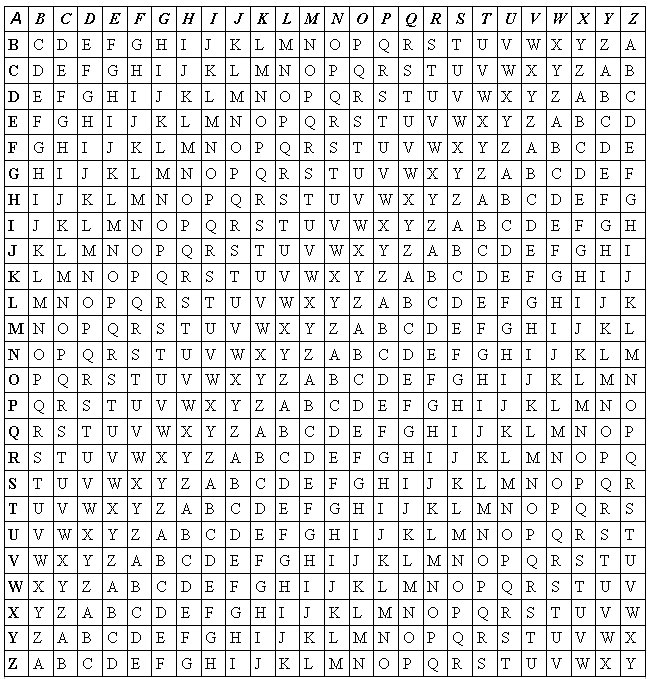
\includegraphics[scale=0.7]{Grafiken/VigenereSquare.jpg}
\caption{Vigenère Quadradt, an der X-Achse ist die Verschiebung und Y-Achse der Klarbuchstabe}
\end{figure}
\subsubsection{Electronic Codebook Modus}
Im ECB Modus werden die einzelnen Blöcke im Blockchiffre Kryptosystem jeweils mit dem selben Schlüssel verschlüsselt und die einzelnen Chiffretexte kombiniert um den gesamten Chiffretext zu bekommen. Die \hyperref[pic:ECBModus]{Entschlüsselung} läuft analog.
Da nicht alle Blöcke die genau vom Kryptosystem geforderte Länge besitzen müssen die Blöcke teilweise mit einer Auffüllfunktion $pad: M^*\rightarrow (M^n)^*$ gefüllt idealerweise sollte eine pad Funktion wieder umkehrbar sein.
Der ECB Modus ist für Klartexte welche in mehrere Blocke augeteilt werden unsicher und sollte nie verwendet werden.\\
Im ECB Modus ist die Ver- und Entschlüsselung parallelisierbar.

\begin{figure}
\centering
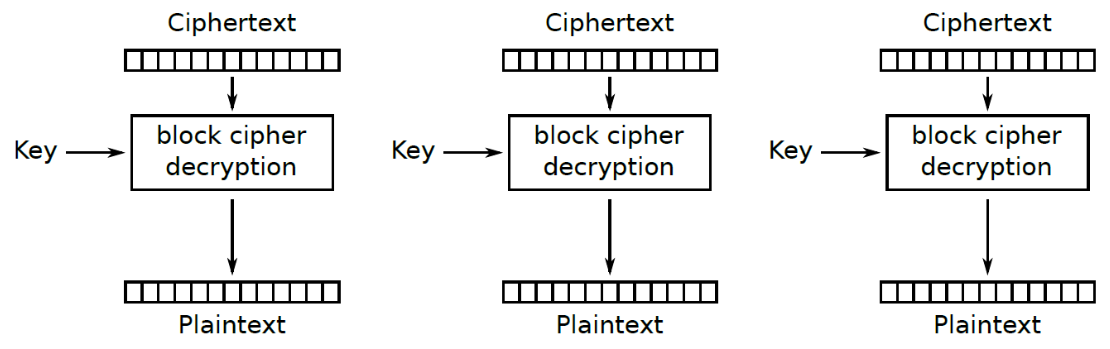
\includegraphics[scale=0.5]{Grafiken/ECBModus.png}
\caption{Entschlüsselung im ECB Modus}
\label{pic:ECBModus}
\end{figure}

\subsubsection{Cipher Block Chaining Modus}
Der CBC Modus ist eine Verbesserung des ECB Modus, da hier für die Ver- und \hyperref[fig:CBCModus]{Entschlüsselung} jeweils der vorherige Block als Rauschen mit dem Klartext verodert wird, sodass auch gleiche Muster im Klartext verschiedene Ergebnisse im Chiffretext produzieren. Dafür erweitern wir das Kryptosystem um die Menge der Zufallswerte $\mathcal{R}$ aus welcher der Initialisierungvektor gewählt wird. Hierbei ist $\mathcal{R}$ nicht geheim und kann unverschlüsselt übertragen werden.\\
Es soll $e(x,k,r_1)\neq e(x,k,r_2)$ gelten. Für die Sicherheit der Verschlüsselung ist wichtig, dass jeder Zufallswert nur einmal verwendet wird.\\
Das erweiterte Kryptosystem heißt \blue{randomisiertes symmetrisches Kryptosystem} und wird als 6-Tupel dargestellt: $(\mathcal{M},\mathcal{K},\mathcal{C},\mathcal{C},\mathcal{R},e^*,d^*)$. Der Definitionsbereich von $e^*$ und $d^*$ wird um $\mathcal{R}$ erweitert.
$$y_i = e(x_i\oplus y_{i-1},k), x_i = d(y_i,k)\oplus y_{i-1} \textrm{ für } i\geq 1$$
\begin{figure}
\centering
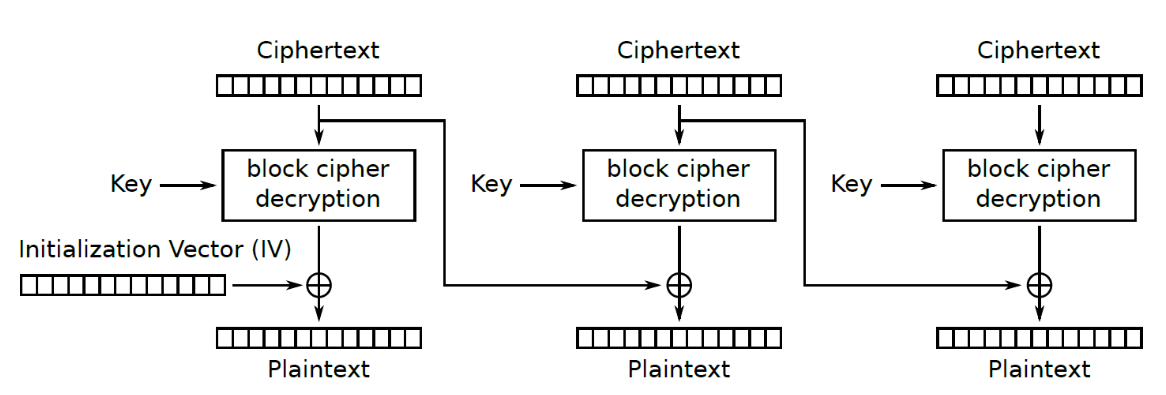
\includegraphics[scale=0.5]{Grafiken/CBCModus.png}
\caption{Entschlüsselung im CBC Modus, bei der Entschlüsselung umgedreht, sodass Parallelisierung unmöglich ist}
\label{fig:CBCModus}
\end{figure}
Die Verschlüsselung ist damit nicht mehr parallelisierbar, aber die Entschlüsselung bleibt es.\\

Damit die Verschlüsselung auch parallelisierbar ist gibt es den \blue{Counter (CTR) Modus} hier wird bei der Verschlüsselung für jeden Block der Initialiserungsvektor mit einem Zählerwert verschlüsselt und erst dann mit dem Klartext verodert. Die \hyperref[pic:CTRModus]{Entschlüsselung} läuft genau gleich ab, nur das hier der Ciffretext verodert wird.\\
\begin{figure}
\centering
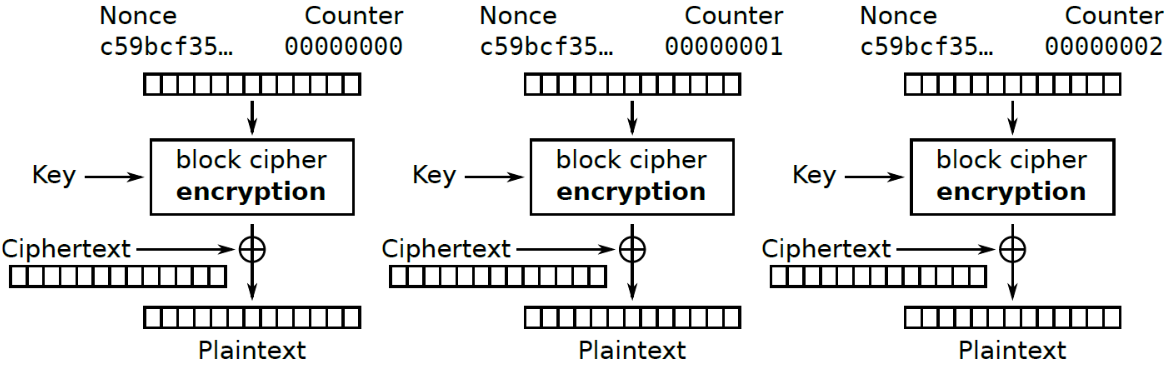
\includegraphics[scale=0.5]{Grafiken/CounterCTRModus.png}
\caption{Entschlüsselung im CTR Modus, Nonce ist der Initialiserungsvektor}
\label{pic:CTRModus}
\end{figure}
Die Wahl des Initialisierungsvektor muss unvorhersagbar sein, das heißt nicht das die Initialisierungsvektoren selber geheim bleiben müssen (die Sicherheit des Chiffretextes garantiert der Schlüssel) sondern dass die Wahl zukünftiger Initialisierungsvektoren nicht vorhersagbar sein dar (sie also von geheimen Informationen abhängen) und ein Angreifer die Wahl nicht beeinflussen kann\footnote{\url{https://tinyurl.com/y5x3bd5j} BSI Seite 76}.\\
Möglichkeiten zur Wahl des Initialisierungsvektor sind:
\begin{itemize}
\item Zufällige Initialisierungvektoren, d.h. eine zufällige Bitfolge der Länge n, hier muss die Bitfolge aber ein Entropie von 95 Bit besitzen ($n\geq95$?)
\item Verschlüsselte Initialisierungsvektoren, wir wählen einen determistisch erzeugten Wert und verschlüsseln ihn mit der einzusetzenden Blockchiffre und Schlüssel, der Chiffretext ist der Initialisierungsvektor
\end{itemize}

Der randomatisierte Zähler wird als eine Funktion $ctr: \mathbb{Z}_2^*\times \mathbb{N}_0\rightarrow \mathbb{Z}_2^n$  definiert welche die basierend auf dem gegebenen Zufallswert eine Erhöhung in unspezifierter Weise ausführt.\\
Mögliche Implementationen umfassen:
\begin{itemize}
\item Einfacher Zähler, welcher den Zufallswert um n erhöht
\item  Die Hälfte der Bits des Zufallswertes sind reserviert und nur die rechte Hälfte der Bits wird erhöht und läuft über\footnote{\url{https://tinyurl.com/y27ga7ew} NST Seite 18ff, Anhang B}
\end{itemize}
Das wiederverwenden des Zufallswertet kompromitiert die Sicherheit der Verschlüsselung, da sobald ein Ciffretext einen Klartext zugeordnet wurde der Schlüssel ermittelt werden kann.\\
Das CTR Modus Kryptosystem wird formal so bezeichnet $((\mathbb{Z}_2^n)^*,\mathbb{Z}_2^n,(\mathbb{Z}_2^n)^*,\mathbb{Z}_2^*,e^*,e^*)$ wobei e und d wie folgt definiert sind:
\begin{align*}
e^*:(\mathbb{Z}_2^n)^*\times \mathbb{Z}_2^m \times \mathbb{Z}_2^n\rightarrow (\mathbb{Z}_2^n)^*, e^*(x_0x_1...x_l,k,r)=y_0y_1...y_l \textrm{ mit } y_i = e(ctr(r,i),k)\oplus x_i\\
d^*:(\mathbb{Z}_2^n)^*\times \mathbb{Z}_2^m \times \mathbb{Z}_2^n\rightarrow (\mathbb{Z}_2^n)^*, d^*(y_0y_1...y_l,k,r)=x_0x_1...x_l \textrm{ mit } x_i = e(ctr(r,i),k)\oplus y_i\\
\end{align*}
\subsubsection{Stromchiffren}
Stromchiffren sind pseudozufällige Schlüsselströme welche aus dem Schlüsselwert generiert werden und zur Ver- und Entschlüsselung mittels xor mit den Klar-/Chiffretext kombiniert werden. Deshalb muss der Schlüssel sicher erzeugt sein, da die Sicherheit des Verfahrens nur davon abhängt, denn ein Pseudozufallszahlengenerator ist deterministisch.\\
Formal wird ein Stromchiffre Kryptosystem so bezeichnet: $(\mathbb{Z}_2^*,\mathbb{Z}_2^k,\mathbb{Z}_2^*,e,d)$ mit der Funktion:
\begin{align*}
keystream: \mathbb{Z}_2^*\times \mathbb{Z}_2^k\rightarrow\mathbb{Z}_2^* \textrm{ mit } |keystream(x,z)|=|x|\\
e(x,z)=d(x,z) = x\oplus keystream(x,z)
\end{align*}
Hierbei liegt es an der Implementation des keystreams ob dieser auch vom ersten Parameter abhängig ist oder ob die Zufallswert nur aus dem Schlüssel erzeugt werden.

\subsection{Asymmetrische Kryptosysteme}
Bei asymmetrischen Kryptosystemen werden zum Ver- und Entschlüsseln zwei verschiedene Schlüssel verwendet. Es gibt also ein Schlüsselpaar aus \blue{öffentlichen Schlüssel},der zum Verschlüsseln verwendet wird und einem \blue{privaten Schlüssel} welcher zum Entschlüsseln verwendet wird.
Als asymmetrisches Kryptosystem bezeichen wir das 7-Tupel: $$(\mathcal{M},\mathcal{K}_s, \mathcal{K}_p,\mathcal{K},\mathcal{C},e,d)$$
Asymmetrische Kryptosysteme sind viel langsamer und benötigen wesentlich größere Schlüssel als symmetrische Kryptographie. Die Kombination beider Verfahren wird als hybride Verschlüsselung bezeichnet, hier wird die Nachricht mit einem symmetrischen System verschlüsselt, die Schlüssel aber über ein asymmetrisches System verschlüsselt, die Nachricht ist hier allerdings nun von der Sicherheit zweier Kroptosystemen abhängig.
\subsubsection{RSA-Kryptosystem}
Das RSA Verfahren beruht auf der Annahme, dass es kein effizientes Verfahren zum Faktorisieren gibt, das Verfahren kann mit Quantencomputern gebrochen werden.
Das Verfahren sollte zur Sicherheit mindestens mit 2048 Bit großen Schlüsseln arbeiten, besser mit 4096 Bit.
\begin{tabbing}
1. \= FormatFormat\= FormatFormatFormatFormat\kill
1.\>Wähle große Primzahlen $p,q$ mit $p\neq q$\\
2.\>Berechne $n=pq$ und $\varphi(n)=(p-1)\cdot(q-1)$\\
3.\>Wähle einen \blue{Verschlüsselungsexponenten} $1\neq e\in \mathbb{Z}_{\varphi(n)}^\times$ so dass ggT$(e,\varphi(n))=1$ gilt\\
4.\>Berechne den \blue{Entschlüsselungsexponenten} $d\in\mathbb{Z}_{\varphi(n)}^\times$, so dass \\
\>\>$d$ das \hyperref[sec:euklid]{multiplikative Inverse} von e ist, d.h.$ed$ mod $\varphi(n)=1$
\end{tabbing}
Hierbei ist $(e,n)$ der öffentliche Schlüssel und $(d,n)$ der private Schlüssel.
Zur Verschlüsselung wird anschließend der Klartext in Zahlenwerte umgewandelt, sodass $c=m^e$ mod $n$ den Chiffretext und $m = c^d$ mod $n$ den Klartext ergibt.\\
Zur Sicherheit sollten anschließend die Werte $p,q,\varphi(n)$ gelöscht werden, da bereits der Besitz eines einzigen davon das Verfahren bricht, aus p bzw. q lässt sich die andere Primzahl berechnen, da das Produkt beider bekannt ist und mit $\varphi(n)$ lässt sich einfach mit dem öffentlichen Schlüssel der private berechnen.\\ Eine häufige Wahl für den public-key e ist die Zahl 65537, da dieser von einigen Autoritäten vorgeben wird und ein guter Mittelwert für die Verschlüsselungsgeschwindigkeit darstellt\footnote{\url{https://tinyurl.com/y7uy76b9} Crypto Stackexchange}.

\newpage
\textbf{Beispielrechnung:}\\
Wir wählen die Primzahlen $p=47$ und $q=59$ und als Nachricht den Wert $m=2345$.
\begin{align*}
n=p\cdot q= 47\cdot 59 = 2773\\
\varphi(n)=(p-1)(q-1)= 46\cdot 58=2668
\end{align*}
Damit haben wir also $\mathbb{Z}_{2668}^\times$ und können z.B. $e=17$ wählen. Damit ergibt sich für d mithilfe des erweiterten euklidischen Algorithmus:
\begin{table}[h!]
\centering
\begin{tabular}{|l|l|l|l|l|}
$\varphi(n)$ & $e$ & $\lfloor\frac{\varphi(n)}{e}\rfloor$ & x & y\\
\hline
2668 & 17 & 156 & -1 & 1-156$\cdot$(-1)=157\\
\hline
17 & 16 & \violet{1} & 1 & \orange{0}-\violet{1}$\cdot$\blue{1}=$-1$\\
\hline
16 & 1 & 16 & \orange{0}& \blue{1}\\
\hline
1 & 0 & & 1 & 0
\end{tabular}
\end{table}\\
Damit ist der $d=157$ und der private Schlüssel also $(157,2773)$ und der öffentliche Schlüssel $(17,2773)$
Damit ergibt sich:
\begin{align*}
c=m^e mod n = 2345^{17} mod 2773 = 2030\\
m=c^d mod n = 2030^{157} mod 2773 = 2345
\end{align*}

\subsubsection{Elgamal-Kryptosystem}
Ein Verfahren was auf der Annahme beruht, dass der diskrete Logarithmus nicht einfach berechenbar ist.\\
Die Schlüsselerzeugung funktioniert wie folgt:\\
1. Wähle eine zyklische\footnote{Sie besitzt einen Erzeuger, sodass $\langle g\rangle:=\{g^n : n\in \mathbb{Z}\}=\mathcal{G}$ (Potenz mit dem gegebenen Verknüpfungsoperator)} Gruppe $\mathcal{G}=(G,\diamond,e)$ mit Erzeuger $g$ und $a\in \{2,...,ord(\mathcal{G})\footnote{Anzahl der Elemente in Gruppe bzw. unendlich}-1\}$, setze $A=g^a$\\
2. Privater Schlüssel ist $(\mathcal{G},g,a)$\\
3. Öffentlicher Schlüssel ist $(\mathcal{G},g,A)$\\

Die Verschlüsselung erfolgt wie folgt:\\
1. Wähle zufällig $r\in \{1,...,ord(\mathcal{G})-1\}$, setze $R = g^r$\\
2. Berechne $K=A^r=(g^a)^r=g^{ar}$ und $C=m\diamond K$\\
3. Sende $e(m,(\mathcal{G},g,A))=(R,C)$\\

Die Entschlüsselung funktioniert wie folgt:\\
1. Berechne $K=R^a=(g^r)^a=g^{ra}=g^{ar}$\\
2. Bestimme $K^{-1}$ in $\mathcal{G}$\\
3. $d((R,C),(\mathcal{G},g,a))=C\diamond K^{-1}=m$

\subsection{Hashfunktionen}
Mittels Hashfunktionen können die \hyperref[item:schutzziele]{Schutzziele Integrität und Authentizität, sowie Nicht-Abstreitbarkeit} gewährleistet werden.\\
Sei $A$ ein Alphabet und $m,n\in\mathbb{N}$ mit $n<m$, dann heißt die Funktion $h: A^m\rightarrow A^n$ \blue{Kompressionsfunktion} und $h: A^*\rightarrow A^n$ Hashfunktion. Diese Funktionen heißen \blue{schwach kollisionsresistent}, falls kein Angreifer in der Lage ist effizient zu einem gegebenen Urbild $x$ einen zweiten Wert $x'$ zu finden der auf den selben Wert abbildet,d.h. $x,x'\in A : x\neq x' \wedge h(x)=h(x')$. Sie heißen \blue{stark kollisionsresitent}, falls es nicht möglich ist irgendeine Kollision effizient zu bestimmen.\\
Anforderungen an kryptographische Hashfunktionen sind:
\begin{itemize}
\item Leicht und schnell zu berechnen
\item \hyperref[def:Einwegfunktion]{Einwegfunktion}
\item (Stark) kollisionsresistent
\item Kleine Änderungen an der Eingabe haben große Änderungen am Hashwert
\end{itemize}
Eine Kompressionsfunktion kann auch als Konkatenation der Verschlüsselungsfunktion von Blockchiffren aufgefasst werden.
\subsubsection{Merkle-Damg\r{a}rd-Konstruktion}
Sei $A$ ein Alphabet, $f: A^{n+m}\rightarrow A^n$ eine Kompressionsfunktion,\\
pad:$A^*\rightarrow (A^m)^*$ eine Auffüllfunktion, $x_0\in A^n$ ein beliebiger Initialisierungsvektor und\\
g:$A^n\rightarrow A^n$ eine Finalisierungsfunktion.\\
Dann ist die Hashfunktion $h: A^*\rightarrow A^n$ für $x\in A^*$ definiert durch
\begin{enumerate}
\item $x_1x_2...x_k=pad(x)$ mit $x_i\in A^m$
\item $h_0=f\left( conc(x_0,x_1)\right)$ und $h_i=f\left(conc(h_{i-1},x_i)\right)$ für $1\leq i\leq k$
\item $h(x)=g(h_k)$
\end{enumerate}
Wobei das Salt oft $x_0=0^n$ als 0-Padding und $g=id_{A^n}$ als Identitätsfunktion gewählt wird.
\begin{figure}
\centering
\includegraphics[scale=0.6]{Grafiken/merkledamgard.png}
\caption{Bei Merkle-Damg\r{a}rd wird jeder Block mit den vorigen Block komprimiert und dann mit g finalisiert}
\end{figure}
\subsubsection{Exkurs: Chosen Target Forced Prefix}
Die Merkle-Dam\r{a}rd-Konstruktion hat gegebenfalls - falls die Kompressionsfunktion $f$ nicht schwach kollisionsresistent ist - Schwächen für Chosen Target Forced Prefix (CTFP) Angriffe, wo ein Angreifer für einen gegebenen Hash $H$ einer nicht umbedingt geheimen Nachricht $N$, aus einem erzwungenen Präfix $P$ kokateniert mit einem frei wählbaren Suffix $S$ eine Nachricht erzeugt, sodass $h(M)=H=h(PS)$ gilt. Hat der Angreifer eine freie Wahl über die möglichen Formulierungen von $P$, sodass deren Bedeutung erhalten bleibt, kann hier nun aus einer signifikant kleineren Menge an Kodierungen ein Suffix $S$ gesucht werden, was den Angriff leichter macht.\\
Darauf aufbauend lässt sich ein Herding-Angriff\footnote{\url{https://eprint.iacr.org/2005/281.pdf} Herding Hash Functions} konstruieren:
\begin{enumerate}
\item Konstruieren einer \hyperref[pic:herdingattack]{Baumstruktur}, sodass für $2^k$ Startblöcke unseres Suffixes die Kanten Strings enthalten, sodass jeweils 2 Knoten zu einem Zwischenhash $h_i$ zusammenlaufen. Dies wird solange wiederholt bis alle Pfade zu einem finalen Hash $H$ zusammenlaufen welcher commited wird. Um eine Stufe abzusteigen werden rund
\item Nach einiger Zeit, wird der zu wählende Präfix $P$ bekannt/gewählt
\item Wir suchen nun einen einzigen Block, sodass wenn dieser an $P$ konkateniert wird einen Zwischenhash in unser Baumstruktur ergibt.
\item Nun werden die Strings bis hin zur Wurzel konkateniert, wodurch eine gefälschte Nachricht entsteht die den selben Hash besitzt wie die unsprünglich committete 
\end{enumerate}

\begin{figure}
\centering
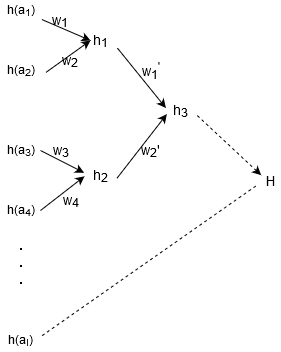
\includegraphics[scale=0.6]{Grafiken/HerdingAttack.png}
\label{pic:herdingattack}
\caption{Dieser Hashbaum gibt Pfade an um aus $2^k$ Hashes den gewünschten Hash durch Konkatenation der Strings zu erreichen.}
\end{figure}

\begin{figure}[h!]
\centering
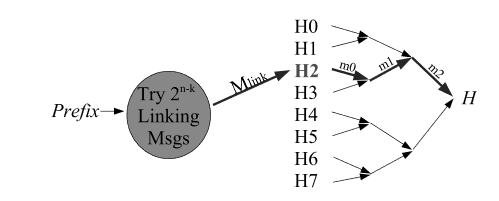
\includegraphics[scale=0.6]{Grafiken/HerdingAttack2_Linking.png}
\label{png:herdinglinking}
\caption{Nachdem ein Linkender String gefunden wurde, kann die gefälschte Nachricht zusammengesetzt werden}
\end{figure}
Ist die Menge an möglichen Präfixen im vorhinein bekannt, so kann die Menge an Starthashes entsprechend dieser Präfixe gewählt werden, wodurch der Aufwand für die Suche des Linkenden Strings gespart wird. Ist die Menge so groß dass nicht alle möglichen Hashkombinationen berechnet werden können, so könnte auch das Risiko einer Entarnung in Kauf genommen werden, wenn ein genügend ähnlicher Präfix verwendet wird. Des weiteren können auch sofern die zu verändernden Stellen innerhalb von abzugrenzenden Blöcken eines Dokumentes liegen, für jede einzelne Stelle eigene alternierende Texte mit den selben Hashes gefunden werden, sodass diese auch ohne eine Baumstruktur vertauscht werden können.
\subsubsection{HMAC-Konstruktion}
Sei $H: \mathbb{Z}_2^*\rightarrow\mathbb{Z}_2^{8n}$ eine Hashfunktion, $opad = (0x5C)^n=(01011100)^n\in \mathbb{Z}_2^{8n}$\\
und $ipad=(0x36)^n=(00110110)^n\in \mathbb{Z}_2^{8n}$, dann definieren wir $HMAC:\mathbb{Z}_2^*\times\mathbb{Z}_2^*\rightarrow\mathbb{Z}_2^*$ als
$$HMAC(x,k)=H\left( conc\left( K\oplus opad, H\left( conc\left( K\oplus ipad,x\right)\right)\right)\right)$$
Dabei ist die Wahl von $K\in\mathbb{Z}_2^{8n}$ von k abhängig:
\begin{itemize}
\item $|k|=8n\Rightarrow K=k$
\item $|k|=m<8n\Rightarrow K = k0^{8n-m}$, d.h. k wird auf Blockgröße aufgefüllt
\item $|k|>8n\Rightarrow K = H(k)$
\end{itemize}
Der Keyed-Hash Message Authentification Code (HMAC) hashed hierbei die Nachricht x, sodass auch bei der Verwendung einer Hashfunktion welche nicht kollisionsresistent ist das Verfahren nicht unsicher wird. Da der Hashwert der Nachricht direkt innerhalb einer Hashoperation berechnet wird, gilt die Grundlage für CTFP nicht, da hier die Berechnung nicht in unterteilten Blöcken funktioniert. $H(x)=H(x')\nRightarrow H(xS)=H(x'S)$\\
Damit ist die HMAC Konstruktion zwar effizient und eine Fälschung einer Nachricht schwierig, um die Authentizität einer Nachricht zu prüfen müssen aber beide Parteien den geheimen Schlüssel kennen um den Hash neu zu bilden und zu prüfen.\\
Varianten des HMAC sind:\\
\blue{HMAC-based One-time Password Algorithmus (HOTP)} verwendet einen Zähler welcher nach jeder Hashgeneration inkrementiert wird und bei der Hashgeneration den Schlüsssel erhöht. Anschließend wird der Hash in einen 6-10 stelligen numerischen Wert umgewandelt welcher auch von Menschen lesbar ist. Die selben Informationen müssen dem Authentifizierenden vorliegen, sodass falls dieser den Hash reproduzieren kann die Nachricht als gültig anerkannt wird. \\
\blue{Time-based One-time Password Algorithmus (TOTP)} verwendet anstelle eines Zählers einen Zeitstempel, funktioniert sonst aber wie HOTP. Um die Ungenauigkeiten nicht synchronisierter Uhren auszugleichen umfasst der Gültigkeitsraum eines TOTP Hashes oft rund 30 Sekunden, bevor der Hash ungültig wird. Das Verfahren kommt vor allem in der 2-Faktor Authentifizierung zum Einsatz.\\
\subsection{Digitale Signaturen}
Signaturen erlauben es die \hyperref[item:schutzziele]{Authentizität, Integrität und Nicht-Abstreitbarkeit} einer Nachricht zu testen bzw. sicherstellen.\\
Ein Angreifer kann keinen Schlüssel generieren, sodass damit für zwei verschiedene Nachrichten die selbe Signatur erzeugt wird.\\
Wir unterscheiden:
\begin{itemize}
\item \blue{Fortgeschrittene elektronische Signatur}
	\begin{itemize}
	\item Signatur ist eindeutig dem Unterzeichner zuordenbar
	\item Ermöglicht Identifizierung des Unterzeichners
	\item Wird unter Verwendung elektronischer Signaturerstellungsdaten erstellt, die der Unterzeichner mit einem hohen maß an Vertrauen unter seiner alleinigen Kontrolle verwenden kann
	\item Nachträgliche Veränderung unterzeichneter Daten muss erkannt werden
	\end{itemize}
\item \blue{Qualifizierte elektronische Signatur}
	\begin{itemize}
	\item Rechtliche Gleichstellung mit handschriftlicher Unterschrift
	\item Eine Signatur welche auf einem von einem Mitgliedsstaat ausgestellten Zertifikat beruht, ist in allen Mitgliedsstaaten gültig
	\end{itemize}	
\end{itemize}

\subsubsection{Wissen und Ziele von Angreifern}
Wie viel Wissen ein Angreifer hat unterscheiden wir mit folgenden Begriffen:
\begin{itemize}
\item \blue{Key-Only Attack}, hier besitzt der Angreifer nur den öffentlichen Schlüssel
\item \blue{Known Signature Attack}, hier sind mehrere Paare von Nachricht und Signatur bekannt
\item \blue{Chosen Message Attack}, der Angreifer kann im Vorfeld für beliebige selbstgewählte Nachrichten die Signatur bekommen
\item \blue{Adaptive Chosen Message Attack}, kann während des Angriffes für beliebig viele selbstgewählte Nachrichten zugehörige Signaturen bekommen
\end{itemize}
Die Ziele eines Angreifers mit folgenden Begriffen:
\begin{itemize}
\item \blue{Existential Forgery}, der Angreifer will ein gültiges Nachricht/Signatur-Paar ermitteln
\item \blue{Selective Forgery}, gültige Signatur zu einzelnen neuen, vor dem Angriff bekannten Nachrichten ermitteln
\item \blue{Universal Forgery}, gültige Signatur zu jedem beliebigen Dokument ermitteln
\item \blue{Total Break}, Angreifer bestimmt den geheimen Schlüssel 
\end{itemize}

Der stärkste Sicherheitsbegriff ist der des \textit{Existential forgery under a chosen message attack}

Ein Signaturschema gilt als \textbf{sicher}, wenn jeder Angreifer nach dem er n Nachrichten signiert hat mit \textbf{sehr hoher Wahrscheinlichkeit} keine Nachricht findet, sodass diese von den ursprünglich n verschieden ist aber die Signatur mit einer davon übereinstimmt

\subsubsection{Signieren mit RSA}

Mittels RSA kann signiert werden, denn die Ver-/Entschlüsselung kommutieren. Dazu wird zusätzlich noch eine Hashfunktion $h: A*\rightarrow \{0,...,n\}$ benötigt.\\
Die Signatur wird wie folgt erstellt: $s=D(h(m),(d,n))=\left( h(m)\right)^d\textrm{ mod }n$\\
Überprüfen lässt sie sich wie folgt: $h(m)=E(s,(e,n))=s^e\textrm{ mod }n$\\

\textbf{Beispiel Signaturvorgang mit RSA:}\\
Signieren:
\begin{enumerate}
\item Schlüsselgenerierung mit $(d,n)=(37313,241103)$ und $(e,n)=(65537,241103)$
\item Alice will die Nachricht $m$ mit $h(m)=164796$ signieren
\item Sie berechnet $s=h(m)^d\textrm{ mod }n=164796^{37313}\textrm{ mod }241103=129335$ 
\end{enumerate}
Verifizieren:
\begin{enumerate}
\item Bob besitzt $(e,n)$, sowie die Nachricht $m$ und ihre Signatur $s=129335$
\item Er berechnet $s^e\textrm{ mod }n=129335^{65537}\textrm{ mod }241103=164796$
\item Er berechnet den Hash der Nachricht $m$
\item Da beide Berechnungen das selbe Ergebnis haben, akzeptiert Bob die Signatur
\end{enumerate}
Eine Signaturerstellung mit RSA ist nur sicher, sofern RSA sicher ist.

\subsubsection{Digital Signature Algorithm}

\textbf{Parametergenerierung:}
\begin{enumerate}
\item Wähle gleichverteilt zufällig eine große Primzahl $q$ (160 Bit, 224 Bit, 256 Bit)
\item Wähle große Primzahl $p$ (1024 Bit, 2048 Bit, 3072 Bit), sodass $q|(p-1)$ gilt
\item Suche ein $g\in\mathbb{Z}_p^\times$ mit ord\footnote{Die Ordnung eines Elementes ist die Zahl ord$(g):=$ inf$\{n\in\mathbb{N}:g^n=e\}\in\mathbb{N}\cup\{\infty\}$}$(g)=q$,d.h. wir wählen $h\in\mathbb{Z}_p^\times$ mit $g:=h^{\frac{p-1}{q}}\textrm{ mod } p \neq 1$.\footnote{ Da $ggT(h,p)=1$ ist, gilt $g\equiv_p h^{\frac{p-1}{q}}\xRightarrow{\text{Kleiner Fermat}}g^q\equiv_p h^{p-1}\equiv_p 1\Rightarrow$ ord$(g)\leq q$.\\ Da $q$ prim ist kann die Ordnung von $g$ kein Teiler von $q$ sein, damit gilt ord$(g)=q$}
\item Die Parameter $p,q,g$ sind öffentlich
\end{enumerate}

\textbf{Schlüsselgenerierung:}
\begin{enumerate}
\item Wähle zufällig $x$ mit $1<x<q$
\item Berechne $y=g^x\textrm{ mod }p$
\end{enumerate}
Dann ist $y$ der öffentliche Schlüssel und $x$ der private Schlüssel.\\
Die Berechnung des privaten Schlüssel aus dem öffentlichen Schlüssel ist eine Instanz des diskreten Logarithmus, und somit nicht effizient lösbar.\\

\textbf{Signieren:}
\begin{enumerate}
\item Wähle $k$ mit $1<k<q$
\item Bestimme $r=(g^k\textrm{ mod }p)\textrm{ mod }q$. Falls $r=0$, beginne von vorne
\item Bestimme $s=k^{-1}\cdot (H(m)+r\cdot x)\textrm{ mod }q$. Falls $s=0$, beginne von vorne
\item Signatur ist das Tupel $(r,s)$
\end{enumerate}
\textbf{Verifikation:}
\begin{enumerate}
\item Ungültig, wenn $0<r<q$ oder $0<s<q$ nicht gilt
\item Berechne $w=s^{-1}$ mod $q$
\item Berechne $u_1=H(m)\cdot w$ mod $q$
\item Berechne $u_2=r\cdot w$ mod $q$
\item Berechne $v=(g^{u_1}\cdot y^{u_2}\textrm{ mod }p)$ mod $q$
\item Akzeptiere die Signatur, falls $v=r$
\end{enumerate}

%%Falls oben mehr Text hin kommt auskommentieren
\newpage

\textbf{Beispiel für DSA}\\
Parametergenerierung:
\begin{enumerate}
\item Wir wählen $q=59$ und $p=709$
\item Mit $h=5$ gilt $g:=5^{\frac{709-1}{59}}\textrm{ mod }709=20 \neq 1$
\item Also sind $(p,q,g)=(709,59,20)$ die öffentlichen Parameter
\end{enumerate}
Schlüsselgenerierung:
\begin{enumerate}
\item Wähle $x=23$ als privaten Schlüssel
\item Bestimme $y=g^x$ mod $p=20^{23}$ mod $709=186$ als öffentlicher Schlüssel
\end{enumerate}

Signieren:\\
Wir besitzen $p=709,q=59,g=20$ und $x=23$, der Hashwert unserer Nachricht ist $H(m)=16$
\begin{enumerate}
\item Wir wählen $k=36$
\item Wir bestimmen $r=(20^{36}\textrm{ mod }709)\textrm{ mod }59=31$
\item Mit $k^{-1}=41$ bestimmen wir $s=k^{-1}\cdot (H(m)+r\cdot x)\textrm{ mod }q=29889\textrm{ mod }59=35$
\item Die Signatur ist damit $(r,s)=(31,35)$
\end{enumerate}

Verifizieren:\\
Es sind $p=709,q=59,g=20,y=186,H(m)=16$ und der Signatur $(r,s)=(31,35)$
\begin{enumerate}
\item $r$ und $s$ sind gültig
\item Wir berechnen $w=s^{-1}$ mod $q=27$
\item Wir berechnen $u_1=H(m)\cdot w$ mod $q=16\cdot 27$ mod $59=19$
\item Wir berechnen $u_2=r\cdot w$ mod $q=31\cdot 27$ mod $59=19$
\item Wir berechnen $v=(g^{u_1}\cdot y^{u_2}\textrm{ mod }p)$ mod $q=(20^{19}\cdot 186^{11}$ mod $p)$ mod $q =31$
\item Da $v=r$ gilt, wird die Signatur akzeptiert
\end{enumerate}

\subsection{Schlüsselverteilung}
\label{sec:Schlüsselverteilung}
Wir unterscheiden verschiedene Schlüssel:\\
\blue{Langzeitschlüssel} haben eine lange Gültigkeit (1 Monat bis 1 Jahr) und werden häufig zur Authentifizierung verwendet.\\
\blue{Kurzzeitschlüssel} bzw. \blue{Sitzungsschlüssel} haben nur eine begrenzte Gültigkeit und minimieren somit das Risiko falls der Schlüssel kompromittiert wird.\\

Ob bei einem asymmetrischen System ein öffentlicher Schlüssel tatsächlich von einer bestimmten Person kommt, kann mithilfe von Zertifkaten welche von einem vertrauenswürdigen Dritten - Public Key Infrastructure (PKI) - ausgestellt werden, verifiziert werden.
Ein solches Zertifikat beinhaltet unter Anderem: Öffentlicher Schlüssel, Name, Gültigkeitszeitraum, Austeller,...\\
Das Zertifikat wird dann mit einer digitalen Signatur des Ausstellers versehen, sodass derjenige der die Authentizität des Schlüssels prüfen will trotzdem noch dem Schlüssel des Zertifikat-Ausstellers vertrauen muss oder eben der nächst \hyperref[pic:Chainoftrust]{höheren Instanz welche den Schlüssel des Zertifikats-Austellers signiert}.

\begin{figure}
\label{pic:Chainoftrust}
\centering
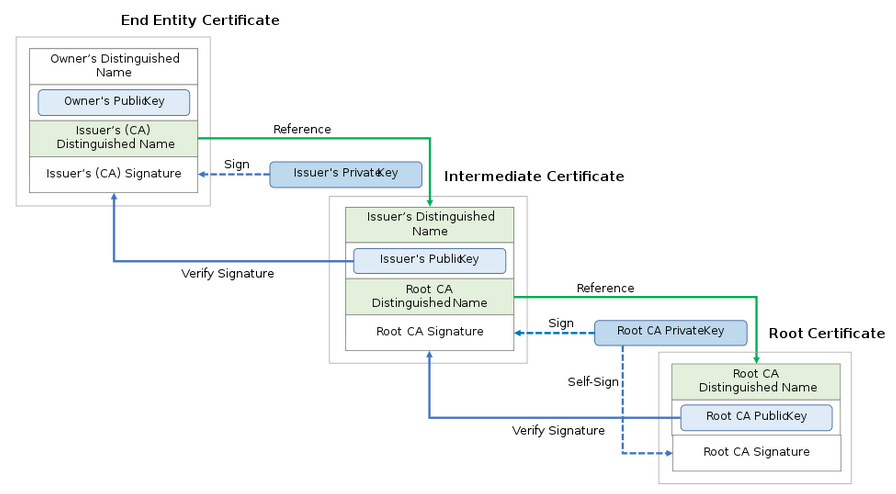
\includegraphics[scale=0.5]{Grafiken/Chain-Of-Trust.png}
\caption{Ein zentralisierter Ansatz ist X.509 als PKI, Root Certificates muss vertraut werden}
\end{figure}

Ein dezentralisierter Ansatz ist PGP (pretty good privacy), hierbei werden Schlüsselbünde versandt, sodass der Empfänger zum einen weiß welchen anderen öffentlichen Schlüsseln der Sender vertraut und dann in seinen bereits vorher empfangenen Schlüsselbändern nachsehen kann ob andere Personen denen er bereits vertraut auch dem Sender vertrauen. Falls dies der Fall ist kann er die neu erhaltenen Schlüssel als vertrauenswürdig speichern, sodass über Zeit ein Web of Trust entsteht wo alle Parteien untereinander ihre öffentlichen Schlüssel kennen. Hierbei ist aber fraglich ob Vertrauen wirklich transitiv ist.\\

Ein Problem bei beiden Ansätzen sind das ein Schlüsselverlust/-kompromittierung dafür sorgt dass die Nachrichten nicht mehr lesbar/geheim sind.\\
Als Lösung für letzteres kann ein Ablaufdatum für Zertifikate festgelegt werden oder mittels Widerrufszertifikaten vorher ausgestellte Zertifikate widerrufen werden.
Diese Widerrufszertifikate können bei X.509 von einem zentralisierten Server ausgestellt werden, wobei auch hier die Vertrauenswürdigkeit und Erreichbarkeit des Servers fragwürdig ist.
Beim Web of Trust können diese durch die Benutzer oder angegebene Parteien erstellt und verbreitet werden. Diese Updates zu verbreiten ist aber ineffizient, sollen alle alles speichern?

\subsection{Schlüsselaustausch}
Beim Man-in-the-middle Angriffsmodel hat der Angreifer vollen Zugriff auf dem Kommunikationskanal. Er kann daher:
\begin{itemize}
\item Nachrichten abfangen
\item Übermittlung von Nachrichten verzögern
\item Nachrichten unterdrücken
\item Nachrichten durch andere Nachrichten ersetzen
\item Nachrichten unter falscher Identität senden
\item Er kann aber keine kryptographische Primitive nicht brechen
\end{itemize}
\begin{figure}
\centering
\label{pic:ManInTheMiddle}
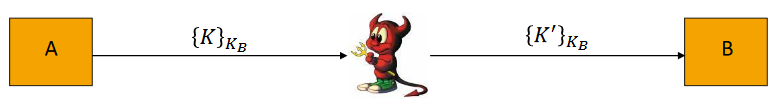
\includegraphics[scale=0.6]{Grafiken/ManInTheMiddle.png}
\caption{Man-in-the-middle Angriff, wo A einen neuen symmetrischen Schlüssel, mit öffentlichem Schlüssel $K_B$ von B verschlüsselt an B sendet, die Chiffre wird vom Angreifer abgefangen}
\end{figure}
Das \hyperref[pic:ManInTheMiddle]{naive Schlüsselaustausch Protokoll} kann um eine PKI erweitert werden, welche die öffentlichen Schlüssel von A und B kennt. A holt von T den öffentlichen Schlüssel $K_B$ von B und verschlüsselt damit den neuen Sitzungsschlüssel und schickt diesem zusammen mit seinem Namen an B. Auch hier kann ein Angreifer die Chiffre abfangen und seinen Schlüssel in Verbindung mit seinem Namen an B senden.

\subsubsection{Needham-Schroeder Protokolle}
Die \textbf{symmetrische Variante} des Protokolls läuft wie folgt ab:
\setcounter{equation}{0}
\begin{flalign}
A\rightarrow T:& A,B,N_A&&\\
T\rightarrow A:& \{ N_A,K,B,\{ K,A\}_{K_B}\}_{K_A}&&\\
A\rightarrow B:& \{ K,A\}_{K_B}&&\\
B\rightarrow A:& \{N_B\}_K&&\\
A\rightarrow B:& \{N_B-1\}_K&&
\end{flalign}
Hierbei sind $N_A$ und $N_B$ zufällig generierte Nonces. Die in Klammern geschriebene Werte werden als eine zusammengesetzte Nachricht mit dem tiefgestellten Schlüssel verschlüsselt. Dabei muss T im Besitz eines geheimen Schlüssels $K_A$ und $K_B$ zum kommunizieren mit jeweils A und B sein.\\

Indem A im ersten Schritt die gewünschten Kommunikationspartner und eine Nonce $N_A$ an den Server sendet kann dieser einen geheimen Sitzungsschlüssel $K$ generieren über den nach Abschluss des Verfahrens eine gesicherte Kommunikation zwischen A und B möglich wird. Damit die im zweiten Schritt von A empfangene Chiffre auch tatsächlich einen neuen Sitzungsschlüssel enthält muss $N_A$ neu sein, da sonst ein Angreifer eine aufgezeichnete Nachricht anstelle von T an A senden könnte um die Verwendung eines alten Schlüssels zu erzwingen. Damit außerdem kein im ersten Schritt der Empfänger nicht durch einen anderen ausgetauscht werden kann ohne das A es bemerkt sendet T auch B erneut zurück. Die innere mit $K_B$ verschlüsselte Chiffre enthält das in Schritt 3 an B gesendete Paket und kann nur von B entschlüsselt werden.\
Damit sich auch B davon überzeugen kann dass der Sitzungschlüssel $K$ neu ist sendet er eine mit K verschlüsselte Nonce $N_B$, welche A dekrementiert und zurücksendet, da $N_B$ neu ist kann auch B sicher sein, dass es sich um keinen Replay-Angriff handelt\footnote{Eine Angriffsform wo ein Angreifer zuvor aufgezeichnete Daten sendet um die Identität des vorherigen Gesprächpartners vorzutäuschen}.\\
Leider obliegt die Schlüsselgenerierung dem Knoten T auch kennt T nun den Sitzungsschlüssel.

\begin{figure}
\centering
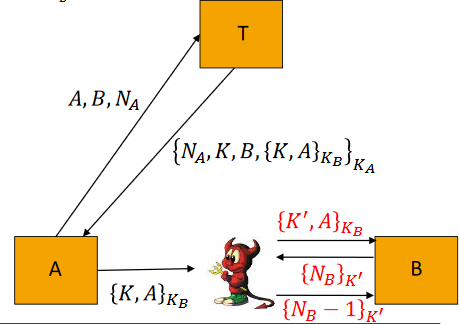
\includegraphics[scale=0.6]{Grafiken/NeedhamSchroederSymmetrisch.png}
\caption{Die symmetrische Variante des Needham-Schroeder-Schlüsselaustausches, falls der Angreifer ein altes Paar $\{K',A\}_{K_B}$ und $K'$ kennt kann der Angreifer die Indentität von A annehmen}
\end{figure}

In der \textbf{antisymmetrische Variante} funktioniert der Datenaustausch wie folgt:
\setcounter{equation}{0}
\begin{flalign}
A\rightarrow T:& A,B&&\\
T\rightarrow A:& \{K_{PB},B\}_{K_{ST}}&&\\
A\rightarrow B:& \{N_A,A\}_{K_{PB}}&&\\
B\rightarrow T:& B, A&&\\
T\rightarrow B:& \{K_{PA},A\}_{K_{ST}}&&\\
B\rightarrow A:& \{N_A,N_B\}_{K_{PA}}&&\\
A\rightarrow B:& \{N_B\}_{K_{PB}}&&
\end{flalign}

Hierbei sind $K_{PA}$ und $K_{PB}$ die öffentlichen Schlüssel von A bzw. B, sowie $K_{ST}$ der private Signaturschlüssel von T.

\subsubsection{Diffie-Hellman-Protokoll}
\label{text:DiffieHellman}
Zu Beginn muss eine Primzahl $p$ und ein Generator $g\in \mathbb{Z}_p^\times$ für eine Gruppe $\mathbb{Z}_p$ gemeinsam gewählt werden. Dann läuft das Verfahren wie folgt ab:
\begin{enumerate}
\item A wählt $a\in\mathbb{N}$ mit $0<a<p$ zufällig und sendet $g^a$ mod $p$ an B
\item B wählt $b\in \mathbb{N}$ mit $<b<p$ zufällig und sendet $g^b$ mod $p$ an A
\item A berechnet $(g^b)^a$ mod $p$
\item B berechnet $(g^a)^b$ mod $p$
\end{enumerate}
Damit haben A und B den selben Schlüssel $g^{ab}$ mod $p$ und können darüber kommunizieren. Ein passiver Angreifer, d.h. ein Angreifer welcher nur den Datenaustausch mithören kann $a$ oder $b$ nicht einfach berechnen.\\
Allerdings wurde früher oft nur eine geringe Menge an Primzahlen für p verwendet, sodass die möglichen Logarithmen vorberechnet werden konnten. Zwei Vorberechnungen deckten $66$\% der IPsec-VPNs und $26$\% der SSH-Server ab.
Bei einem MitM-Angriff kann der Angreifer damit parallel zwei DH-Protokolle laufen lassen und so Schlüssel selber wählen.
Als Lösung hierfür können die Nachrichten signiert werden \blue{authenticated DH/Station-to-Station-Protokoll}.\\

Für das Station-to-Station-Protokoll (STS) müssen beide Parteien einen Signaturschlüssel $sk_A$ und $sk_B$ besitzen und die Zertifikate der Schlüssel sind beiden bekannt. Wir bezeichnen $K=g^{ab}$ mod $p$
\setcounter{equation}{0}
\begin{flalign}
A\rightarrow B: & g^a\textrm{ mod }p&&\\
B\rightarrow A: &g^b\textrm{ mod }p ,\{sig(sk_B,(g^a\textrm{ mod }p,g^b\textrm{ mod }p))\}_K&&\\
A\rightarrow B: & \{sig(sk_A,(g^a\textrm{ mod }p,g^b\textrm{ mod }p))\}_K &&
\end{flalign}

\subsection{Ausblick}

\subsubsection{Integritätsschutz mit Verschlüsselung}

Man unterscheidet zwischen Authenticated Encryption (AE), wo Daten verschlüsselt werden und diese Chiffre nicht manipulierbar sein soll, und Authenticated Encryption with Associated Data (AEAD), wo zusätzlich zu AE noch Metadaten unverschlüsselt übertragen werden sollen deren Integrität auch sichergestellt werden muss.\\
\begin{figure}[h!]
\centering
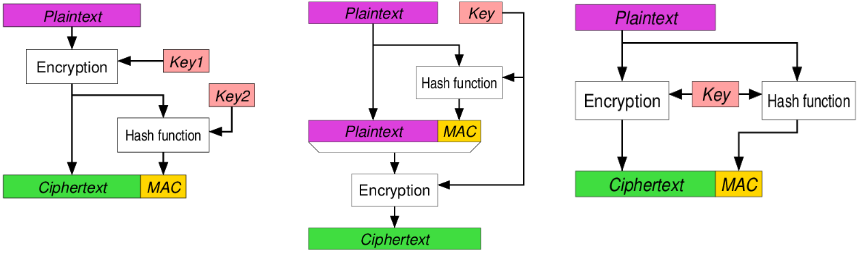
\includegraphics[scale=0.7]{Grafiken/AEKombiMAC.png}
\caption{Dies sind AE-Verfahren: EtM ist sicher, MtE und E\&M sind nur bedingt sicher}
\end{figure}

Ein AEAD Verfahren ist Galois/Counter-Mode welches mit 128 Bit Blockchiffren arbeitet und Integritätsschutz für verschlüsselte Daten bietet.\\
\begin{itemize}
\item $GCTR_K(ICB,X_1||X_2||...||X_n^*)=Y_1||Y_2||...||Y_n^*$
	\begin{enumerate}
	\item Falls X leer ist, gibt es zurück
	\item Setzte den ersten Zählblock $CB_1=ICB$ auf den Initialisierungswert
	\item Für i = 1 bis n sei $CB_i= inc_{32}(CB_{i-1})$
	\item Für i = 1 bis n-1 sei $Y_i=X_i\oplus CIPH_K(CB_i)$ für i = n wir bis zum Blockende xored, sodass $Y_n^*$ selbe Länge wie $X_n^*$ hat.
	\end{enumerate}
\item $GHASH_H(X_1||X_2||...||X_m)=Y_m$
	\begin{enumerate}
	\item Sei $Y_0=0^{128}$
	\item Für $i=1,...,m$ sei $Y_i=(Y_{i-1}\oplus X_i)\bullet H$, wobei $\bullet$ der Multiplikation im Galois Körper $\mathbb{F}_{2^{128}}$ entspricht.
	\end{enumerate}
\end{itemize}
\begin{figure}
\centering
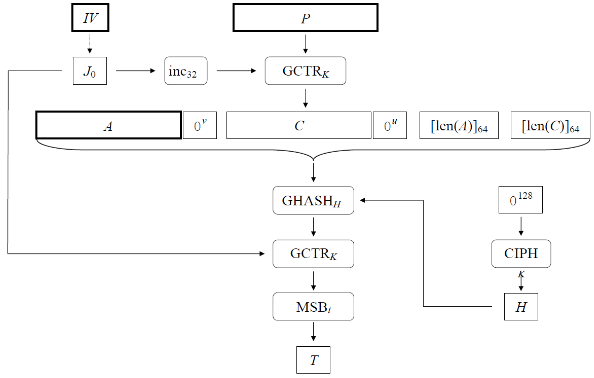
\includegraphics[scale=0.9]{Grafiken/GCMArchitektur.png}
\caption{Im GCM-Verfahren wird}
\end{figure}

\subsubsection{Secret Sharing}
Man möchte Informationen so verschlüsseln, dass man zum Entschlüsseln eine gewisse Gruppe von Leuten zusammenarbeiten müssen. Eine Variante ist das $(t,n)$-Schwellenwert-Kryptosystem wo mindestens $t$ von insgesamt $n$ Shareholdern zusammenarbeiten müssen um eine Nachricht zu entschlüsseln.\\

Ist Geheimhaltung wichtiger als Verfügbarkeit sollte $t$ nah an $n$ gewählt werden, anders herum sollte $t$ möglichst klein aber größer als $\frac{n}{2}$ gewählt werden.\\
Um ein $(t,n)$-Kryptosystem zu konstruieren wendet man $\begin{pmatrix}n\\t\end{pmatrix}$-mal das $(t,t)$-Schwellenwert-Kryptosystem an. Damit bekommt jeder Shareholder $\begin{pmatrix}n-1\\t-1\end{pmatrix}$ Shares, um jeden möglichen Ausfall von $(n-t)$ Shareholdern abzudecken.\\
Hierfür nehmen wir an, dass der Dealer vertrauenswürdig und der Kommunikationskanal zwischen Dealer und Shareholder, und Shareholder und Combiner sicher sind. Außerdem nimmt man an dass zumindest die Hälfte aller Shareholder ehrlich ist.\\

\textbf{Shamirs Secret Sharing Protokoll:}
Wir haben einen Schlüssel $k$ und wollen das mindestens $t$ Shareholder zusammenarbeiten müssen um ihn wiederherzustellen. Sei $n$ die Anzahl an Shareholdern.\\
Wahl der Shares:
\begin{enumerate}
\item Dealer wählt Primzahl $p$ mit $p>k$ und $p>n$
\item Dealer wählt $t-1$ Koeffizienten $a_1,a_2,...,a_{t-1}\in \mathbb{Z}_p$
\item Dealer wählt Polynom $f(x)=k+a_1\cdot x+a_2\cdot x^2+...+a_{t-1}\cdot x^{t-1}$ mit $f(0)=k$ und $a_{t-1}\neq 0$
\item Die Shares sind $\{s_1,s_2,...,s_n\}=\{(1,f(1)),(2,f(2)),...,(n,f(n))\}$
\end{enumerate}
Entschlüsselung:
\begin{enumerate}
\item $t$ der $n$ Shareholder geben ihre Shares dem Combiner
\item Der Combiner versucht das Polynom wieder herzustellen (Lagrange-Interpolation)
	\begin{enumerate}
	\item Definiere $l_i=\prod_{j=1,j\neq i}^t\frac{x-x_j}{x_i-x_j}$
	\item Bemerke $l_i(x_k)=\left\lbrace\begin{array}{lr}1,&\textrm{wenn }i=k\\0,&\textrm{wenn }i\neq k\end{array}\right.$
	\item Definiere $L(x)=\sum_{i=1}^ty_i\cdot l_i(x)$
	\item Bemerke $L(x_i)=y_i$ für alle $1\leq i\leq t$
	\end{enumerate}
\end{enumerate}
Das Verfahren ist perfekt sicher, selbst wenn man $t-1$ Shares besitzt, sind alle Schlüssel gleich wahrscheinlich. Sofern $t$ gleich bleibt, können weiter Shares ohne Probleme hinzugefügt werden. Bei einem neuen $t$ kann das Verfahren mit dem selben $k$ einfach erneut ausgeführt werden.

\subsubsection{Post-Quanten-Kryptographie}
\textbf{Grovers Algorithmus} ist ein Algorithmus für Quantencomputer welcher unsortierte Datenbanken in $\mathcal{O}(\sqrt{n})$ Schritten durchsucht. Also findet er Schlüssel der Länge $n$ in $\mathcal{O}(\sqrt{2^n})$ Schritten. Eine einfache Lösung für symmetrische Kryptographie ist eine Vergrößerung (mindest Verdopplung) der Schlüssellänge.\\ 

\textbf{Shors Algorithmus} hat zum Ziel $n$ effizient zu faktorisieren.
\begin{enumerate}
\item Wähle $a\leq n$ zufällig
\item Wenn ggT($a,n$)$\neq$1, so gebe ggT($a,n$) aus
\item Finde die Periode $r$ von $a$ modulo $n$, d.h. die kleinste natürliche Zahl $r$, so dass $a^r\equiv 1$ mod $n$
\item Wenn $r$ ungerade ist, oder $a^{\frac{r}{2}} + 1\equiv 0$ mod $n$, so starte erneut bei Schritt 1
\item Nun gilt $a^r-1=kn$
\item Gib also ggT($a^{\frac{r}{2}}\pm 1,n$) als Lösung zurück
\end{enumerate}

Der \textbf{Algorithmus von Deutsch} kann entscheiden ob eine Funktion $f: \{0,1\}\rightarrow\{0,1\}$ konstant ist oder nicht, ohne die unterspezifizierte Funktion zwei mal auswerten zu müssen.\\

In der \textbf{hashbasierte Kryptographie} wird der Hash der Schlüssels als öffentlicher Schlüssel verwendet und sein Urbild als privater Schlüssel, denn die Urbildberechnung ist auch für Quantencomputer schwer.\\
Lamport-(Diffie-)Einmal-Signaturverfahren (Schlüsselerzeugung):
Alice will eine Nachricht der Länge 256 Bit signieren.
\begin{enumerate}
\item Alice wählt (zufällig und gleichverteilt) 256 Paare von Zahlen, jeweils 256 Bits lang (privater Schlüssel)
\item Sie hasht nun jede Zahl, die Hashs sind der öffentliche Schlüssel
\end{enumerate}
Signierung:
\begin{enumerate}
\item Für jedes Bit der Nachricht wählt Alice je nach Wert des Bits entweder die erste oder die zweite Zahl aus einem Paar ihres privaten Schlüssels
\item Die gewonnene Zahlenfolge ist ihre Signatur
\end{enumerate}
Verifizierung:\\
Bob hasht jede Zahl der Signatur und prüft, ob die Ergebnisse zu den jeweils passenden Zahlen des öffentlichen Schlüssels passen.\\

Der Schlüssel darf nur einmal verwendet werden, da ein Angreifer von jeder Signatur lernt und aus Signaturen bekannter Nachrichten auch Signaturen für neue Nachrichten erzeugen kann. Zum Beispiel kann aus den Signaturen zu Nachricht $0010$ und $0111$ auch die Signatur zu $0110$ und $0011$ erzeugt werden.\\
Der öffentliche Schlüssel und die Signatur sind im Verhältnis zur Nachrichtenlänge sehr lang.

\subsubsection{Zero-Knowledge Beweise}

Bei Zero-Knowledge Beweisen möchte ein Beweiser $P$ einen Verifizierer $V$ davon überzeugen, dass er ein Geheimnis kennt, ohne dabei irgendwelche Informationen über das Geheimnis preiszugeben. Außerdem soll ein außenstehender Dritter nicht davon überzeugt werden, dass der Beweiser das Geheimnis kennt.\\

In einem Kryptosystem in dem der öffentliche Schlüssel zwei isomorphe Graphen $(G_0,G_1)$ sind und der private Schlüssel der Isomorphismus $\pi$ zwischen den beiden. Der Beweiser $P$ ist im Besitz von $\pi$ und möchte einen Verifizierer $V$ im Besitz des öffentlichen Schlüssels überzeugen, dass er $\pi$ kennt.

\begin{enumerate}
\item $P$ wählt ein zufälliges $a\in\{0,1\}$ und eine zufällige Permutation $\rho$ auf dem Graphen. Damit berechnet er $H:=\rho(G_a)$ und sendet $H$ an $V$ (Commitment)
\item $V$ wählt ein zufälliges $b\in\{0,1\}$ und fordert $P$ auf ihm eine Permutation $\sigma$ mit $H=\sigma(G_b)$ zu senden (Challenge)
\item $P$ wählt nun die Permutation wie folgt$\sigma:=\left\lbrace\begin{array}{lr}
\rho, & \textrm{falls }a=b\\
\rho\circ \pi^{-1},& \textrm{falls }a=0\wedge b=1\\
\rho\circ \pi, &\textrm{falls }a=1\wedge b=0
\end{array}\right.$ und sendet sie an $V$
\item $V$ enpfängt $\sigma$ und prüft ob $H=\sigma(G_b)$ gilt
\end{enumerate}
$P$ kann nur dann immer ein richtiges $\sigma$ senden, wenn P im Besitz von $\pi$ ist. Das Protokoll muss also hinreichend oft wiederholt werden um $V$ wirklich zu überzeugen (Wahrscheinlichkeit von $1-2^{-n}$)
\section{IT-Sicherheit}

\subsection{Zugriffskontrolle}

\begin{figure}[h!]
\centering
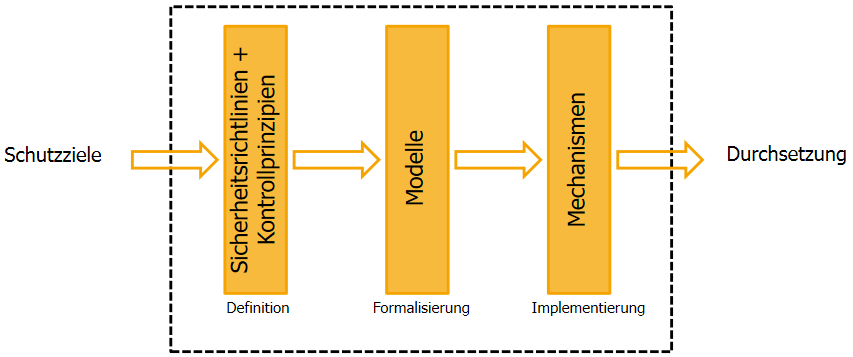
\includegraphics[scale=0.5]{Grafiken/Sicherheitsmodellentwicklung.png}
\caption{Kontrollprinzipien sollen die Einhaltung der Sicherheitsrichtlinien gewährleisten und werden durch Modelle abstrahiert. Mechanismen implementieren diese Modelle.}
\end{figure}
Drei Modelle zur Zugriffskontrolle sind:\\

\begin{itemize}
\item Benutzerbestimmbare Zugriffkontrolle (DAC)
	\begin{itemize}
	\item Eigentümer ist für die Zugriffberechtigungen zu Objekten selbst verantwortlich
	\item Rechte werden für einzelne Objekte vergeben
	\item Objektbezogene Sicherheitseigenschaften, aber keine systemweiten
	\item Fast alle Betriebssysteme unterstützen DAC
	\end{itemize}
\item Rollenbasierte Zugriffskontrolle (RBAC)
	\begin{itemize}
	\item Berechtigungen für Rollen statt Benutzer (MS Active Directory)
	\end{itemize}
\item Systembestimmte Zugriffkontrolle (MAC)
	\begin{itemize}
	\item Systembestimmte (regelbasierte) Festlegung von Sicherheitseigenschaften
	\item Benutzerdefinierte Rechte werden durch systembestimmte überschrieben
	\end{itemize}
\end{itemize}

\subsubsection{Benutzerdefinierte Zugriffskontrolle}
Dieses Modell ist einfach zu implementieren und intuitiv, flexibel einsetzbar.\\
Es gibt allerdings keine formale Garantien für den Informationsfluss, die Rechtevergabe/-rücknahme relativ komplex. Ein beschränkter Zugriff auf bestimmte Teile ist schwierig zu implementieren. Außerdem ist eine Rechtevergabe am Admin vorbei möglich.\\

Dargestellt wird ein DAC als eine Zugriffsmatrix. Formal geschrieben als:
\begin{tabbing}
asdgkjaskjahsfdjkngasjkdhafh\= hajsfjh\=\kill
Menge von Objekten: \> \>   $O$\\
Menge von Subjekten: \>   \>    $S$\\
Menge von Rechten: \>\>$R$ z.B. $R = \{\textrm{read, write, execute, own}\}$\\
Matrix bestimmt Abbildung \>\> $M: S\times O\rightarrow P(R)$
\end{tabbing}
Da in einer Matrixrepräsentation viele Zellen leer bleiben wird eine Access Control List (ACL) verwendet um die Matrixeinträge zu speichern. In dieser stehen Tupel aus dem Prozess/Nutzer mit seinen entsprechenden Rechten.\\
Beispielsweise: $ACL(Datei1)=\{(Prozess1, \{read, write\}),(Prozess5,\{owner,execute\})\}$\\
\begin{figure}
\centering
\includegraphics[scale=0.7]{Grafiken/Unix-ACL.png}
\caption{UNIX speichert die Rechte von Objekten in solchen Einträgen, okal kodiert. Jede Datei kann somit nur einen Besitzer haben}
\end{figure}
Das ist eine objektbezogene Sicht der Zugriffsmatrix, eine andere Variante ist die subjektbezogene Sicht. Hier speichert man für alle Subjekte eine Liste von Objekten samt Zugriffsrechten.\\
Alle Rechte eines Nutzers sind effizient bestimmbar, aber die Rechte an einem spezifischen Objekt schwierig.\\
Beispielsweise: $CL(Prozess3)=\{(Datei2,\{owner, execute\}), (Prozess1,\{signal\})\}$

\subsubsection{Rollenbasierte Zugriffskontrolle}
Hier werden die Rechte an Gruppen vergeben denen Subjekte zugeordnet sind.
Die Rollenmitgliedschaften sind im Vergleich zu DAC leicht zu verändern und unterstützt dynamischen und statischen Ausschluss, sowie Sitzungen (Sessions) sodass nicht alle Rollen gleichzeitig aktiv sind.\\
Formal schreibt man:
\begin{tabbing}
asdgkjaskjahsfdjkngasjkdhafh             \= hajsfjh\=\kill
Menge von Subjekten: \> \>   $S$\\
Menge von Rollen: \>   \>    $R$\\
Menge von Zugriffsechten: \>\>$P$\\
Zuordnung Benutzer $\rightarrow$ Rollen:\>\>$sr: S\rightarrow \mathcal{P}(R)$\\
Zuordnung Rolle $\rightarrow$ Rechte:\>\>$pr: R\rightarrow \mathcal{P}(P)$
\end{tabbing}
Eine Sitzung ist eine Relation $session\subseteq S\times \mathcal{P}(R)$ und modelliert die ''aktive'' Zuordnung von Subjekten auf Rollen. Ein Subjekt kann auch nicht aktive Rollen besitzen.\\
Mit der partiellen Ordnung $\leq\subseteq R\times R$ können wir Rollen nach ihren Rechten ordnen, sodass $R_i\leq R_j$ bedeutet, dass $R_j$ alle Rechte von $R_i$ hat und ggf. noch mehr.\\

Die Funktion $active: S\rightarrow \mathcal{P}(R)$ bildet auf alle aktiven und nach $\leq$ untergeordneten Rollen eines Subjekts ab.\\
Mit $member: R\rightarrow \mathcal{P}(S)$ bildet auf die Menge Subjekte an welche die gegebene Rolle hat.\\
Das Prädikat $exec: S\times P\rightarrow \mathbb{B}$ gibt an ob ein Subjekt aktuell eine Berechtigung hat.\\

In einer RBAC Implementierung muss immer gelten, dass ein Subjekt nur in den Rollen aktiv sein kann, in denen es Mitglied ist und darf nur die Rechte der aktiven Rollen besitzen.\\

Rollentrennung kann statisch mit $SSD\subseteq R\times R$ ausgeschlossen werden, definiert als: $$\forall R_i,R_j\in R,\forall s\in S :\left(s\in member(R_i)\wedge s\in member(R_j)\right)\Rightarrow (R_i,R_j)\not\in SSD$$
Dynamischen Ausschluss definiert man mit $DSD\subseteq R\times R$ wie folgt:
\begin{align*}
\forall R_i,R_j\in R,&\forall s\in S :\\
&(s\in member(R_i)\wedge s\in member(R_j)\wedge \{R_i,R_j\}\subseteq active(s))\Rightarrow (R_i.R_j)\not\in DSD
\end{align*}
RBAC ist eine Erweiterung von DAC falls $pr=M$ gilt. 

\subsubsection{Systembestimmte Zugriffskontrolle}
Dieses Modell beschäftigt sich mit dem Informationsfluss mittels Zugriffsrechten, welche z.B. mit Multi-Level Security überwacht werden.\\

Das Bell-La Padula Modell erweitert die Zugriffsmatrix $M$ um ein Zugriffskontrollsystem, indem es jedem Subjekt $s$ und jedem Objekt $o$ eine Sicherheitsmarkte (label) \textbf{L}  ($vertraulich<geheim<streng$ $geheim$) zuordnet.\\
Außerdem benötigen wir zum erstellen von Sicherheitsklassen \textbf{SC}$=L\times \mathcal{P}(C)$ noch Sicherheitskategorien \textbf{C} welche die Zuständigkeiten modellieren.\\
Jedem Subjekt wird eine Sicherheitsklasse (Ermächtigung) und jedem Objekt eine Sicherheitsklasse (Einstufung) zugewiesen.\\
Auf SC definieren wir eine partielle Ordnung $\leq$:\\ 
$\forall (l,c),(l',c')\in SC:(l,c)\leq (l',c')\Leftrightarrow l\leq l'\wedge c\subseteq c'$\\

Die Sicherheitseigenschaften von Mandatory Access Control sind:
\begin{itemize}
\item \textbf{Simple-security-Property} (no read up Regel)
	\begin{itemize}
	\item Lesezugriff/Ausführung nur erlaubt falls $read\in M(s,o)\wedge SC(o)\leq SC(s)$
	\end{itemize}
\item \textbf{*-Property} (no write down-Regel)
	\begin{itemize}
	\item Append nur erlaubt falls: $append\in M(s,o)\wedge SC(s)\leq SC(o)$
	\item Read-Write nur erlaubt falls: $read-write \in M(s,o)\wedge SC(s)=SC(o)$
	\end{itemize}
\item \textbf{Strong Tranquility Regel}
	\begin{itemize}
	\item Keine Änderung der Subjekt-Clearance oder der Objekt-Classification zur Systemlaufzeit
	\end{itemize}
\end{itemize}
Nachteile des Bell-La Padula Modells sind, dass Daten tendenziell höher klassifiziert werden, Subjekte müssen möglicherweise blind schreiben (nur append). Außerdem können keine verdeckten Kanäle modelliert werden.
Dafür ist das Modell einfach zu implementieren und bildet herarchische Informationsflüsse nach.
\begin{figure}
\centering
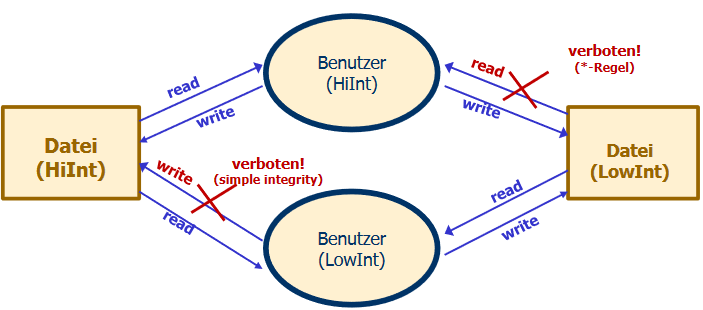
\includegraphics[scale=0.8]{Grafiken/BibaModell-MAC.png}
\caption{Als duale Modellzu Bell-La Padula sichert das Biba Modell die Integrität von Daten}
\end{figure}
\subsection{Authentifizierung}

Wir definieren folgende Begriffe:
\begin{itemize}
\item Identität, als eine Menge von Attributen
\item Authentisierung: Bereitstellung von Unterlagen, die es ermöglichen, die Identität zu prüfen
\item Authentifizierung: Prüfung und Echtheitsbezeugung der Unterlagen zu Identitätsfeststellung
\item Autorisierung: Gewährung/Verwehrung von Rechten 
\end{itemize}

Ansätze zur Authentifizierung sind:
\begin{itemize}
\item Authentifizierung durch Wissen (z.B. PIN, Passwort, krypt. Schlüssel)
\item Authentifizierung durch Besitz (z.B. Smartcard, Token, SIM-Karte)
\item Authentisierung durch Merkmale (z.B. Biometrie)
\end{itemize}
Verschiedene Ansätze werden normalerweise zu einem Mehrfaktorverfahren kombiniert.\\
Bei der \textbf{einseitigen Authentifizierung} authentisiert sich eine Partei A gegenüber einer anderen Partei B (B authentifiziert A). Zum Beispiel Authentifiziert sich ein Nutzer gegenüber eines PC.\\
Bei der \textbf{wechselseitigen Authentifizierung} authentifizieren sich zwei Parteien gegenseitig. Zum Beispiel Online-Banking bei Verwendung von Zertifikaten.

\subsubsection{Authentisierung durch Wissen}

Die gängigste Methode sind Passwörter, welche üblicherweise als Hashwert gespeichert und durch Salts gegen Offline-Attacken weiter geschützt werden können.\\
Probleme sind:
\begin{itemize}
\item Schwache Passwörter (''dictionary attack'')
\item Benutzer verwenden gleiches Passwort bei verschiedenen Servern
\item Manche UNIX-Tools (telnet, ftp) übertragen Passwörter im Klartext
\item NIS, YP übertragen Hashes (''Offline Attacke'')
\end{itemize}
Besser wäre ein Authentifizierungsverfahren welches die nicht Übertragung eines Passwortes erfordern würde.\\
Arten Passwörter zu übertragen:
\begin{itemize}
\item Plaintext: Ein passiver Angreifer kann alles mitlesen
\item Plaintext, TLS geschützt: Angreifer auf Datenbank erlangt alle Passwörter
\item Hash, TLS geschützt: Angriff mit Rainbowtable, da bei eindeutigen Hashalgo. das selbe Passwort für alle Nutzer den selben Hash erzeugt
\item Hash mit Salt, TLS geschützt: Angriff mit Rainbowtable gibt keinen Geschwindigkeitsgewinn, da der Hash nun nicht mehr allein vom Passwort abhängt.
\end{itemize}
Authentifizierung durch Wissen kann auch mit Challenge-Response-Verfahren (CHAP) funktionieren.
\begin{enumerate}
\item Server sendet Challenge $c$
\item Nutzer verwendet Integritätsschutzverfahren auf Nachricht $m:=c$
\item Server prüft ob Nachricht $m=c$ und prüft Authentizität via Verfahren
\end{enumerate}
Wie \href{figure:CHAP}{hier} zu sehen ist, muss Bob ebenfalls das Passwort speichern um $c$ zu verifizieren. Auch wenn $K_{ID}=h(passwort)$ gesetzt wird braucht ein Angreifer in diesem Fall nur $K_{ID}$. Auch muss der Klartextraum von RAND groß sein, damit ein Angreifer keine bereits benutzte Challenge wiederverwenden kann (Replay-Attack).\\
Das Verfahren beweist Bob nur dass Alice sich authentisieren möchte, wenn authentifizierte Daten übertragen werden sollen, muss die Integrität des Kommunikationskanals geschutzt werden (Man-in-the-middle Angriff).

\begin{figure}[h!]
\centering
\label{figure:CHAP}
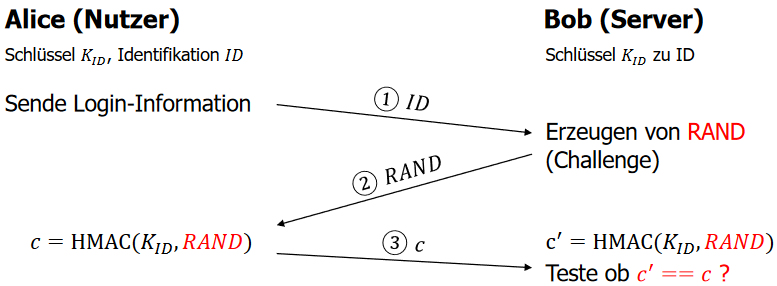
\includegraphics[scale=0.7]{Grafiken/Callenge-Response-Verfahren.png}
\caption{Beide Parteien kennen den gemeinsamen Schlüssel $K_{ID}$, anstelle von HMAC kann auch eine Verschlüsselungsfunktion verwendet werden}
\end{figure}

\subsubsection{Authentisierung durch Besitz}

Nutzer authentifizieren sich mit Tokens welche statisch - ein gespeichertes Geheimnis (Passwort), oder dynamisch - Geheimnis wird zur Berechnung von Authentifizierungs-Informationen genutzt (z.B. CHAP mit SmartCard mit Kryptoprozessor).\\
Token können als Hardware (Schlüssel, SmartCard, Transponder) oder Software (Cookie, Client-Zertifikat) vorliegen.\\

Probleme sind
\begin{itemize}
\item Diebstahl
	\begin{itemize}
	\item Nutzung des Tokens durch zusätzliche Authentifikation sichern
		\begin{itemize}
		\item Software-Crypto: Privaten Schlüssel mit Passwort verschlüsseln
		\item Hardware-Crypto: Token mit Pin
		\end{itemize}
	\item Nutzung mit mit zusätzlichem zweiten Faktor
	\end{itemize}
\item Extraktion der kryptographischen Schlüssel (Kopie)
	\begin{itemize}
	\item Schwachstellen in Tokenfirmware
	\item Side-Channel Angriffe
	\end{itemize}
\end{itemize}

\subsubsection{Authentisierung durch Merkmale}

Anforderungen:
\begin{itemize}
\item \textbf{Universalität:} Jede Person besitzt das Merkmal
\item \textbf{Eindeutigkeit:} Merkmal ist für jede Person verschieden
\item \textbf{Beständigkeit:} Merkmal ist unveränderlich
\item quantitative \textbf{Erfassbarkeit} mittels Sensoren
\item \textbf{Performanz:} Genauigkeit und Geschwindigkeit
\item \textbf{Akzeptanz} des Merkmals beim Benutzer
\item \textbf{Fälschungssicherheit}
\end{itemize}

Die Erkennung läuft in zwei Prozessen, dem \textbf{Enrollment}, d.h. der Registrierung eines Benutzers, und der \textbf{Verifikation}, d.h. der Erfassung und dem Vergleich mit im Enrollment erfassten Daten.\\

Die Verifikation ist immer fehlerbehaftet:
\begin{itemize}
\item False positives: Unberechtigter wird authentifiziert (FAR) $\rightarrow$ Sicherheitsproblem
\item False negatives: Berechtigter wird abgewiesen (FRR) $\rightarrow$ Probleme bei Akzeptanz, Benutzbarkeit
\item FAR und FRR können durch Hinzunahme von Merkmalen gesteuert werden
\item Equal Error Rate, wenn Anzahl an FAR und FRR gleich sind
\item Meist ungeprüfte Hersteller-Angaben
\end{itemize}

Einzelne feine Punkte in Fingerabdrücken bezeichnet man als Minutien. Gemeint sind Verzweigungen, Endpunkte, etc. jeweils mit (relativen) Koordinaten und Winkeln\\
Deren Muster scheint eindeutig zu sein. Minutien können allerdings durch schlechte Abdrücke fehlen. Bei der Verifikation werden vorhandene Minutien mit jenen die beim Enrollment extrahiert wurden verglichen.\\
Biometrie birgt Datenschutzprobleme, da es Rückschlüsse auf medizinische Daten (Venenmuster) und Gesundheitszustand ermöglicht. Anstelle von Merkmalen sollten lediglich Referenzdaten gespeichert werden aus denen keine Rekonstruktion möglich ist.\\

Sensoren können durch künstliche Fingerabrücke, Klone durch hochauflösende Fotos oder Gewaltkriminalität (abgeschnittener Finger) getäuscht werden.\\
Biometriedaten sind nicht (DNA) bzw. nur begrenzt (Fingerabdruck, Iris) widerrufbar.
Wenn Kopien prinzipiell erstellt werden können, stellt die Kompromittierung eines Lesegerätes die Authentifizierung aller anderen in Frage.

\subsubsection{Kerberos}

Ziel von Kerberos ist die zentrale Authentifizierung von Subjekten (Principals), sodass keine separate Authentisierung bei Dienstnutzung erforderlich ist (Single-Sign-on).\\
Jede Domäne besitzt ein Key Distribution Center (KDC) welches aus einem Authentification Server (AS), welcher Principals seiner Domäne authentifiziert, und einem Ticket Granting Server (TGS), welcher Tickets als Identitätsausweis ausstellt.\\
Basis der Authentifizierung sind Pre-Shared Secrets zwischen KDC und Principal, d.h. das KDC kennt die Secrets aller Netzwerkteilnehmer.\\

Ein vom AS ausgestelltes Ticket Granting Ticket (TGT) beinhaltet:\\
$T_{C,S}= (S,C,addr,timestamp,lifetime,K_{C,S})$
\begin{align*}
S & \quad\textrm{Name des Servers}\\
C & \quad\textrm{Name des anfordernden Clients}\\
addr &\quad \textrm{IP-Adresse des Clients}\\
timestamp &\quad  \textrm{aktuelle Zeit}\\
lifetime &\quad \textrm{Lebenszeit des Tickets}\\
K_{C,S} &\quad \textrm{Sitzungs-Schlüssel für Kommunikation zwischen $C$ und $S$}
\end{align*}

\begin{figure}
\centering
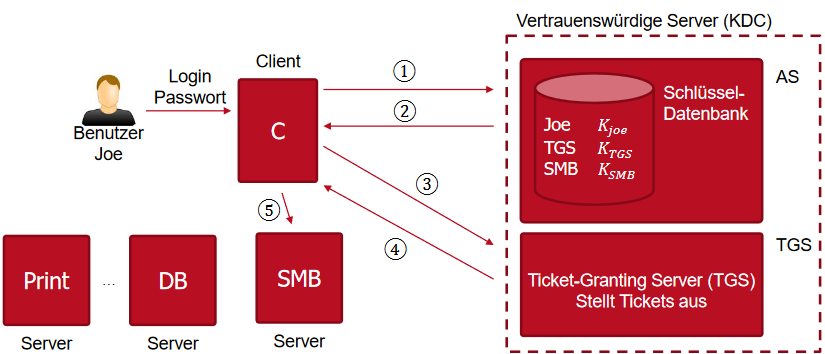
\includegraphics[scale=0.7]{Grafiken/Kerberos-Login.png}
\caption{Loginverfahren bei Kerberos. Nummerierung wie \hyperref[expl:Kerberos-Login]{hier}}
\end{figure}
Der Login funktioniert wie folgt:\\
\label{expl:Kerberos-Login}
Joe gibt Passwort auf lokalem Client C ein, $K_{joe}:= Hash(Passwort)$ wird generiert.
\setcounter{equation}{0}
\begin{flalign}
Joe\rightarrow AS: & \{timestamp\}_{K_{joe}},Joe,N_1,TGS\\
AS\rightarrow Joe: & \{K_{joe,TGS}\}_{K_{joe}},\{TGT\}_{K_{TGS}}\\
Joe\rightarrow TGS: & \{A_{joe}\}_{K_{joe,TGS}},\{TGT\}_{K_{TGS}},SMB,N_2\\
TGS\rightarrow C: & \{K_{joe,SMB},N_2\}_{K_{joe,TGS}},\{T_{joe,SMB}\}_{K_{SMB}} \\
C\rightarrow SMB: & \{A_{joe}\}_{K_{joe,SMB}},\{T_{joe,SMB}\}_{K_{SMB}}\\
SMB\rightarrow C: & \{timestamp+1\}_{K_{joe,SMB}}
\end{flalign}
Hierbei sind $N_1,N_2$ Nonces und $A_{joe}=(Joe,IP-Addr,timestamp)$ der Authenticator ist.
Der sechste Schritt ist optional falls wechselseitige Authentifizierung gewünscht ist.\\
Wenn der AS $\{timestamp\}_{K_{joe}}$ entschlüsseln kann und der Zeitstempel in den letzten 5 Minuten liegt, wird ein Ticket-Granting-Ticket TGT (beinhaltet $K_{joe,TGS}$) ausgestellt.\\
Joe kann nach Empfangen von (2) den Sitzungsschlüssel mit TGS entschlüsseln und den zweiten Teil in (3) an TGS senden sodass TGS sicher mit Joe kommunizieren kann. Außerdem teilt Joe TGS mit, für welchen Dienst er ein Ticket möchte.\\

Wenn TGS den Authenticator erfolgreich überprüft hat, sendet er in (4) einen Sitzungsschlüssel $K_{joe,SMB}$ für Kommunikation zwischen Joe und SMB, sowie ein Ticket für SMB.\\
Joe kann nun das Ticket beim SMB-Server benutzen.\\

\textbf{Angriffe auf Kerberos:}\\

Beim Offline Cracking wird Übertragung (1) abgefangen und $\{timestamp\}_{K_{joe}}$ versucht zu entschlüsseln. Sollte das Ergebnis des Entschlüsselns die Form eines Zeitstempels haben, wird eine Checksum erzeugt und mit der des tatsächlichen Pakets verglichen. Stimme beide überein ist das Passwort gefunden, sonst wird das nächste ausprobiert.\\

Overpass-the-hash, hier kann ein Angreifer sich gegenüber Kerberos als ein bestimmter Nutzer ausgeben, falls er den Hash eines Nutzers kennt ($K_{joe}$ kann auch der Hash des Passwortes sein, wie \hyperref[figure:CHAP]{hier}).\\

Pass-the-Ticket, hier kennt der Angreifer ein Ticket des Nutzers und nutzt dieses um im Namen des Nutzers auf Dienste zuzugreifen. Angriff beginnt ab (3)\\

Golden Ticket, hier stellt der Angreifer sich selbst ein TGT aus, wobei er den Masterkey des Domain Controllers besitzt. Dadurch kann er in (3) ein sein TGT einfügen und kann so vom TGS Zugriff auf jeden Dienst anfordern.\\

Silver Ticket, der Angreifer kennt den Hash/Key eines Application Servers und kann damit im Namen des Servers Zugriff auf alle Dienste anfordern, auf die auch der Server zugriff hat.
Dabei tritt er nicht mit dem Domain Controller in Kontakt

\subsection{Software Security}

\subsubsection{Malware}

Malware kurz für Malicious Software bezeichnet verschiedene Typen:
\begin{itemize}
\item Spyware/Adware
	\begin{itemize}
	\item Ausspähen von persönlichen Daten
	\item Werbedienste installieren
	\end{itemize}
\item Trojanisches Pferd
	\begin{itemize}
	\item Software die in vermeintlich sicherer Software versteckt ist
	\item besitzt versteckte Funktionalitäten um die Nutzer auszuspähen
	\end{itemize}
\item Computervirus
	\begin{itemize}
	\item Programme, die ihren eigenen Code in ''Wirtsprogramme'' einfügen und sich dadurch verbreiten
	\end{itemize}
\item Computerwurm
	\begin{itemize}
	\item Selbstreplizierend
	\end{itemize}
\item Rootkits
	\begin{itemize}
	\item Software welche sich vor Antimalware Software versteckt. (z.B. durch Verändern von Systemdateien)
	\end{itemize}
\item Ransomware/Erpressungssoftware
	\begin{itemize}
	\item verschlüsselt Daten um diese gegen Lösegeld wieder freizugeben
	\end{itemize}
\end{itemize}
Beispiel Trojaner:\\
Thompson's Compiler ist ein modifizierter C Compiler welcher bei der Übersetzung von Tools wie /bin/login bekannte Passwörter akzeptiert. Wird ein neuer Compiler mit dem modifizierten übersetzt, wird der selbe Schadcode in den neuen eingefügt. Der modifizierte Quellcode wird gelöscht und der modifizierte Compiler bereitgestellt.\\

Beispiel Wurm:\\
Win32/Sasser nutzte eine Buffer Overflow Schwachstelle im LSASS Dienst aus um sich auf das Zielsystem zu kopieren. Angekommen scannt er nach weiteren verwundbaren Zielen. Die Schadfunktion war das unregelmäßige Herunterfahren des Computers.\\

\textbf{Viren}\\
Viren bestehen typischerweise aus 3 Phasen:
\begin{enumerate}
\item Insertion phase
\item Execution phase
\item Replication
\end{enumerate}

Bekannte Virentypen sind \textbf{Executable infectors} welche Code im Wirtsprogramm einfügen und den Kontrollfluss entsprechend verändern. Was der Virus kann von externen Faktoren abhängig sein.\\
Diese Arten lassen sich mit Checksummen ausfindig machen.\\

\textbf{Encrypted viruses} verschlüsseln den tatsächlichen Virus code und nur die Entschlüsselungsroutine kann erkannt werden.\\

\textbf{Polymorpic viruses} verändern ihren Code während der Replikation um Erkennung durch statische ''Virensignaturen'' zu verhindern. Hierzu werden gängigerweise Instruktionen durch aquivalenten Code ersetzt.\\

Erkennungsmöglichkeiten für Viren sind statische Virensignaturen, welche die Signaturen von Daten mit den Signaturen bekannter Viren abgleichen. Das ''Window of vulnerability'' liegt hierbei zwischen der Erstellung der Malware und der Veröffentlich der Signatur.\\
Einfache Änderungen am Virus können bereits eine neue Signatur erfordern.\\

\textbf{Sandboxing} hier wird ein Programm in einer VM ausgeführt um sich dessen Verhalten anzusehen. Mittlerweile können Viren aber erkennen ob sie in einer Sandbox ausgeführt werden oder nicht (Abrufen nicht vorhandener Webseiten). Entsprechend wird Schadsoftware ausgeführt oder nicht.\\
Bei der \textbf{dynamische Analyse} wird das Programm decompiliert und verdächtige Codestellen untersucht.\\
Natürlich kann auch mittels heuristischer Herangehensweise nach Viren gesucht werden.

\textbf{Würmer}\\
Würmer sind Programme die sich automatisch über das Netz selbst verbreiten. Geschieht dies ohne Nutzerinteraktion spricht man von ''wormable'' Schwachstellen.\\
Die Ausbreitung von Würmern verläuft exponenntiell, bis die erreichbare Menge von verwundbaren Zielsystemen betroffen ist.\\

\textbf{Phishing}\\
Das Vortäuschen einer authentischen Email/Website mit dem Ziel Daten abzugreifen.
Als Spear Phishing oder Dynamit Phishing bezeichnet man eine zielgerichtete Variante des Phishings welches Informationen über das Ziel verwendet um eine höhere Erfolgsquote zu erreichen, d.h. einen Anhang oder Link zu öffnen. Teilweise sind Fragmente echter (alter) Emails enthalten.

\subsubsection{Buffer Overflow}

Buffer Overflow sind Schwachstellen in klassischen kompilierten Programmen, bei denen aufgrund fehlender Eingabevalidierung Daten überschrieben oder Code ausgeführt werden kann.
Falls die Eingabe über das Netzwerk erfolgt können darüber Würmer eingeschleust werden.\\

Gegenmaßnahmen sind:\\
\textbf{Address Space Layout Randomisation} (ASLR), randomatisiert die Funktionsadressen, sodass ein Angreifer diese nicht vorhersehen kann.\\
\textbf{Stack Canaries} legt einen Prüfwert auf den Stack, sodass ein Überschreiben des RIP auch den Canary überschreibt, sodass das Programm sicherheitshalber abgebrochen wird.\\
\textbf{Non-executable Stack} verhindert das Daten auf dem Stack als Code ausgeführt wird.\\

\begin{figure}[h!]
\centering
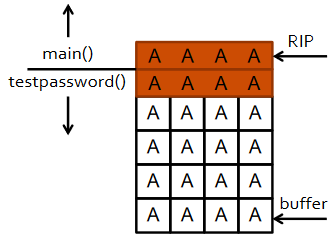
\includegraphics[scale=0.8]{Grafiken/StackSmashing.png}
\caption{Werden zu große Daten auf den Stack geschrieben wird die Rücksprungadresse (RIP) überschrieben und das Programm crashed, da die Adresse nicht existiert}
\end{figure}
Kennt der Angreifer die Adresse der passwortgeschützen Methode kann er mit dieser die RIP überschreiben, sodass diese Aufgerufen wird ohne das Passwort zu kennen.

\subsection{Web Security}


\textbf{Clientseitig:}\\
Schutz der Verbindung mit HTTPS als TLS-gesicherte Verbindung sichert die Vertraulichkeit und Integrität. Authentifikation mittels Zertifikaten garantiert das die aufgerufene Seite authentisch ist. Hierbei unterscheidet man Extended Validation wo die Identität des Serverbetreibers  geprüft wurde. Das ist ein aufwendiger und teurer Prozess. Alternativ gibt es Domain Validation wo überprüft wurde ob der Websitebetreiber Besitzer der Domäne ist, was einfach und schnell, aber weniger sicher ist. Denn die Domain Validation sichert nur das die Domäne stimmt, nicht das die Seite korrekt/sicher ist. Bei Domain Validation wird üblicherweise von der Certification Authority (CA) verlangt dass der Serverbetreiber eine Challenge auf seiner Webseite teilt, sodass die CA feststellen kann dass er tatsächlich der Besitzer der Domain ist.\\
Hierbei kann aber bereits eine bösartige/unzuverlässige CA das System korrumpieren.

Weitere Schutzmechanismen sind:
\begin{itemize}
\item Same-Origin Policy (SOP) untersagt clientseitigen Skriptsprachen auf Objekte anderen Ursprungs als des aufgerufenen Webservers zuzugreifen
\item Cross-Origin Resource Sharing (CORS), eine Variante von SOP welche Corss-Origin-Requests unter bestimmten Bedingungen erlaubt
\item Content Security Policy (CSP) soll Cross-Site-Scripting und Angriffe durch Einschleusen von Daten in Webseiten verhindern soll
\item Frame Sicherheit, durch die Überlagerung von Websiteinhalten führen Nutzer bestimmte Aktionen aus
\item Cookie Security
\item Web Tracking
\item Private Browsing Konzepte
\end{itemize}

\begin{figure}[h!]
\centering
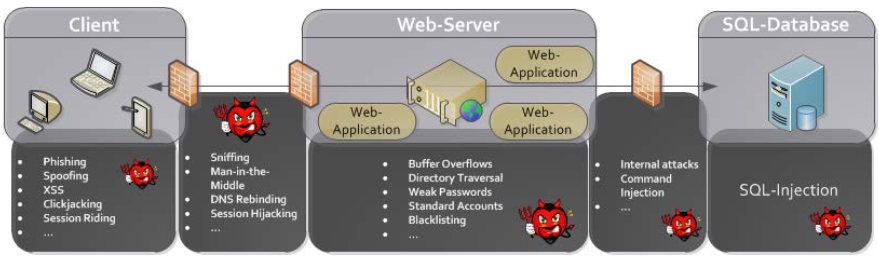
\includegraphics[scale=0.65]{Grafiken/AngriffeWebanwendung.png}
\caption{Verschiedene Angriffsmöglichkeiten auf die einzelnen Teile des Datenaustausches bei Webanwendungen}
\end{figure}

\subsubsection{SQL Injection}

SQL Injections bezeichnet das Einschleusen von SQL Befehlen mittels geschickter Nutzereingaben. Dies passiert meist falls nicht ausreichend geprüfte Nutzereingaben an die Datenbank weitergegeben werden.\\

Dabei werden die Abfragen so verändert, dass aus einer Texteingabe ausgebrochen wird, sodass weiter SQL Befehle an den eigentlichen Befehl angehängt/eingefügt werden.\\
Alle Befehle nach dem Zeichen \# werden ignoriert. Viele Datenbanken erlauben keine multiple statements, d.h. mehrere unabhängige Befehle in einer Zeile.

Gegenmaßnahmen sind 
\begin{itemize}
\item parametrisierte Abfragen mit gebundenen, typisierten Parametern, wo die Nutzereingaben als Parameter in ein vorbereitetes Statement eingefügt wird
\item Benutzung von gespeicherten parametrisierten Abfragen
\item ''Least privilege'' Verbindungen, d.h. der Anwendung so wenige Rechte wie möglich einräumen
\end{itemize}

\subsubsection{Cross Site Scripting (XSS)}

Cross Site Scripting führt Scripte auf dem Rechner des Opfers aus, indem ein Angreifer schadhaften JavaScript Code in eine HTML Seite einschleust.\\

Persistent XSS bezeichnnet XSS wo die Eingabe vom Server gespeichert wird und später ausgegeben und von (anderen) Clients ausgeführt.\\

Bei Non-Persistent/Reflected XSS wird die Eingabe direkt ausgegeben und vom selben Client ausgeführt. Die Eingabe ist zum Beispiel Teil der URL, d.h. der Angreifer sendet eine vorbereitete URL an den Nutzer.

Zum Beispiel kann in den Befehl $<?php$ echo \$\_GET[''name''] $?>$ mittels des URL Anhangs: ?name=$\cdots$ beliebiger Code eingefügt werden.\\

Es muss also jede Nutzereingabe vorgefiltert werden, bevor sie in HTML genutzt werden kann. Dabei sind Blacklists von nicht erlaubten Zeichen nicht effizient realisierbar, da Zeichen viele äquivalente Representationen haben.

\subsection{Netzwerkgrundlagen}

\begin{figure}[h!]
\centering
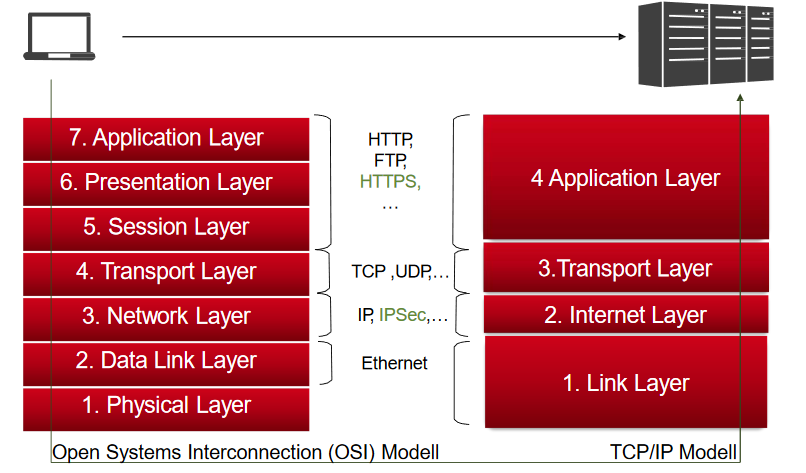
\includegraphics[scale=0.6]{Grafiken/OSI-TCPIP.png}
\caption{OSI und TCP/IP Modell}
\end{figure}
Die Application Layer stellt Funktionen für netzbasierte Software zur Verfügung. Das heißt die HTTP, FTP und SMTP Protokolle liegen auf dieser Ebene.\\

Das Presentation Layer kovertiert die Daten in ein für alle Seiten verständliches Format, außerdem werden die Daten komprimiert und verschlüsselt/entschlüsselt. Zum Beispiel die Konvertierung von ASCII nach ASN.1.\\

Das Session Layer authentifiziert/authorisiert den Benutzer, erstellt und beendet Sitzungen, d.h. beim Aufruf einer Webseite werden z.B. der Download von Text und Bildern in getrennten Sessions geführt. Auch hier werden wieder Daten ver- und entschlüsselt.\\

Das Transport Layer teilt die Daten in Segmente auf welche die Sendereihenfolge und den Service bestimmten.
D.h. jedes Segment bekommt eine Segment- und eine Portnummer zugeteilt.
Auch Fehlererkennung mittels Checksummen wird hier gemacht, genauso die Flusskontrolle, d.h. Anpassung der Bandbreite.\\ 

Das Network Layer versieht jedes Segment mit einer IP-Adresse. Die Daten werden zum Beispiel mit IPSec verschlüsselt. Router arbeiten auf dieser Ebene.\\

Das Data Link Layer verbindet zwei Netzwerkgeräte (Hop-Verbindung mit MAC), Switches entscheiden ob Paket durchgeleitet werden.\\

Im Physical Layer werden Daten in physikalische Signale konvertiert (elektrische Impulse, Lichtimpulse, Funk).\\

Im TCP Modell funktioniert die Identifikation wie folgt:\\
\begin{tabular}{lccc}
1. & Link Layer & MAC-Adresse: & 00:15:fe:23:d4:ce\\
2. & Internet Layer & IP-Adresse:& 130.83.22.1\\
3. & Transport Layer & Port/Protokoll:& 80/TCP  
\end{tabular}\\

MAC-Adressen haben folgenden Aufbau: AA:BB:CC:DD:EE:FF.\\
Dabei haben sie folgende Bedeutung:\\

\begin{tabular}{|c|c|c|}
\hline
Bit & Wert & Bedeutung\\
\hline
 1 & 0 & Individuelle Adresse eines Netzwerkadapters (Unicast)\\
 1 & 1 & Zieladresse für eine Gruppe von Stationen (Multicast)\\
\hline
 2 & 0 & gloabal eindeutige Adresse\\
 2 & 1 & Lokal zugewiesen (nicht umbedingt einzigartig)\\
 \hline
 3 - 24 & & Herstellerkennung\\
 \hline
 25 - 48 & & Gerätekennung\\
 \hline
\end{tabular}\\

Ein IP-Subnetz wird durch die Subnetzmaske definiert welche festlegt, dass alle mit 0-Bits gekennzeichneten Stellen vom Administrator frei vergeben werden können. Die Netzwerk ID ist die niedrigststellige Adresse, die Broadcastadresse die höchstwertige Adresse.\\
Die erste nutzbare IP Adresse wird üblicherweise als Gateway verwendet.\\
In der CIDR Notation wird die Anzahl an 1-Bits in der Subnetzmaske als Anzahl hinten an die Netzwerk ID angehängt, d.h. 172.16.0.0/12.\\

Der Port ist ein 16-Bit Anhang an die IP-Adresse um Prozesse und Services zu identifizieren.\\

\begin{tabular}{|c|c|}
\hline
Port Nummer & Dienst\\
\hline
25 & SMTP\\
80 & HTTP\\
143 & IMAP\\
443 & HTTPS\\
\hline
\end{tabular}

\subsubsection{Spoofing}

\label{txt:spoofing}
MAC-Adressen können leicht gefälscht werden und bieten daher keine sichere Zugriffskontrolle, randomized MACs erleichtern aber anonymes Surfen.\\
IPv4 Adressen werden mit dem Address Resolution Protocol (arp) und IPv6 Adressen werden mit dem Neighbor Discovery Protocol zu MAC Adressen aufgelöst. Da arp Zustandslos ist kannn Eve einfach behaupten eine bestimmte MAC Adresse zu haben (\textbf{ARP Spoofing}).\\

IP Adressen werden über das \textbf{Dynamic Host Configuration Protocol (DHCP)} vergeben. Hierbei fordert Alice mittels Broadcast beim DHCP Server eine IP Adresse an. Der Server sendet anschließend die neue IP-Adresse an Alice.\\
Beim \textbf{DHCP Spoofing} gibt sich Eve als DHCP Server aus und vergibt an Alice eine eigens gewählte IP Adresse. Falls die IP Adresse nicht im Netz liegt ist Alice nicht erreichbar, falls es sich um eine Gateway Adresse handelt führt Eve einen Man-in-the-middle Angriff durch.\\
Eine Gegenmaßnnahme ist DHCP Snooping das im lokalen Netz nur vertrauenswürdige DHCP-Server akzeptiert.\\

Um eine Domain zur zugehörigen IP-Adresse aufzulösen fragt Alice beim DNS Server nach (sofern noch nicht gecashed), dieser sendet ihr die passende IP-Adresse zu. Sollte der DNS Server die Adresse nicht kennen, fragt er beim nächst höhergelegenen DNS Server.\\
Eve kann sich allerdings auch als DNS Server ausgeben und eine falsche IP Adresse an Alice senden.
Die falsche Adresse wird dann von Alice gecashed (\textbf{Cash Poisoning}).\\
Als Gegenmaßnahme können nur authentisierte DNS Antworten per DNSSEC akzeptiert werden.

\subsubsection{Denial of Service}

Bei DoS Angriffen wird der Zielserver durch zu viele Anfragen überlastet, sodass er nicht mehr oder nur sehr eingeschränkt verfügbar ist.\\
Ein DoS Angriff geht hierbei nur von einem Rechner aus.\\
Bei Distributed DoS (DDoS) Angriffen sind mehrere infizierte Rechner (Botnet) beteiligt.\\

Das \textbf{Internet Control Message Protocol (ICMP)} erlaubt es Informations- und Fehlermeldungen des Netzwerks auszutauschen. Der ping Befehl ist Teil dieses Protokolls.\\
Beim \textbf{Ping of Death (PoD) Angriff} werden miskonfigurierte ICMP Nachrichten an den Server gesendet um ihn abstürzen zu lassen.\\
Beim \textbf{Smurf Attack (Broadcast Attack)} wird mittels einem ping an die Broadcast Adresse dafür gesorgt, dass alle Netzteilnehmer eine Antwort an die mitgegebene Antwort-Adresse (Server) senden. Als Gegenmaßnahme kann ping Broadcast verboten werden.\\

Das \textbf{Transmission Control Protocol} (TCP) besteht aus drei Interaktionen. Erst sendet der Nutzer eine SYN Nachricht an den Server. Der Nachricht bestätigt den Erhalt mittels einer SYN-ACK Nachricht. Anschließend ist der Verbindungsaufbau abgeschlossen sobald der Server vom Nutzer eine Acknowledge Nachricht ACK erhält.
Die Verbindung wird offen gehalten bis der Server ACK empfängt.\\
Beim \textbf{SYN-Flood Angriff} werden so viele SYN Anfragen ohne ACK Bestätigung an den Server gesendet, bis dieser aufgrund zu vieler offenen Verbindungen keine weiteren mehr anbieten kann. Als Gegenmaßnahme kann in SYN Cookies die Antwortsequenznummer der Verbindung kodiert werden, sodass nach eingegangenem ACK die SYN Anfrage rekonstruiert werden kann.\\
Ähnlich zum Smurf Attack wird bei der \textbf{SYN-ACK Flood (SYN Reflection Attack)} eine SYN Anfrage mit manipulierter Antwortadresse an alle Teilnehmer eines Netzes gesendet, sodass sie SYN-ACK antworten an das Ziel senden. Als Gegenmaßnahme könnnen SYN-ACKs durch die Firewall gefiltert werden.

\subsubsection{Firewalls} 

Firewalls schützen gegen Angriffe über das Netzwerk welche über die selbe Ebene auf der sie liegen geführt werden. Das heißt Application oder Proxy Firewalls schützen vor Angriffen basierend auf Anwendungen. Sie liegen auf dem Application Layer (TCP/IP).\\
Netzwerk-Firewalls hingegen operieren auf dem Transport Layer (TCP/IP) und schützen vor Angriffen auf UDP/TCP/ICMP.\\
Solche Netzwerk-Firewalls sind entweder zustandslos, d.h. sie entscheident basierend auf einer statischen Liste von Regeln welche Pakete durchgelassen und welche blockiert werden.\\
Zustandsbasierte Paketfilter hingegen entscheiden dynamisch basierend auf dem Verbindungsstatus welche Pakete zur Verbindung gehören und welche blockiert werden.\\

Mittels iptables kann unter Linux Netzwerk-Firewalls konfiguriert werden.\\
Der Aufbau ist hierbei:
\begin{lstlisting}
iptables -A INPUT -p icmp --src 172.16.0.0/12 -j ACCEPT
iptables -A INPUT -p icmp --icmp-type echo-request -j DROP
\end{lstlisting}
Intrusion Detection Systeme (IDS) unterucht auf Netzwerkebene den Inhalt und meldet verdächtige Kommunikation (z.B. Bytecode von Viren, Shellcode). Intrusion Prevention Systeme (IPS) kann verdächtige Kommunikation blockieren oder ändern. Die Übergänge zwischen Firewall und IDS/IPS sind fließend.

\subsection{DNS}

\begin{figure}[h!]
\centering
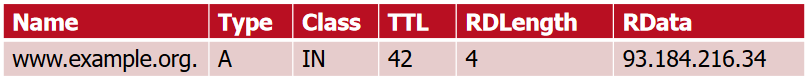
\includegraphics[scale=0.5]{Grafiken/DNS-Record.png}
\label{pic:DNS-Record}
\caption{Beispiel eines DNS Records}
\end{figure}

Domain Name System (DNS) übersetzt Hostnamen in IP-Adressen. Die Auflösung funktioniert durch eine global verteilte Datenbank. Jeder Domainbereich wird von einer einzigen Autorität verwaltet. Die Autorität ist der Domain Registrar oder ein Unternehmen.\\

Die DNS Records werden in dem \hyperref[pic:DNS-Record]{hier} angegebenen Format gepeichert.
Die Felder haben die folgende Bedeutung:\\

\begin{tabular}{|l|c|}
\hline
Bezeichnung & Bedeutung\\
\hline
Name & Identifikator der Hierarchie. . am Ende repräsentiert Wurzel der Hierarchie\\
Type & Datentypbezeichner, gibt das Format von RData vor siehe auch \hyperref[tab:RecordType]{hier}\\
Class & Klassenbezeichner des Netzes heute nur ''IN'' für Internet\\
\hline
TTL & Time to live, Verfallsdatum der Gültigkeit des Wertes ab Ausgabe\\
RDLength & Länge des RData Felds in Bytes\\
RData & Im DNS abgelegte Wert zum Schlüssel (Name, Class, Type)\\
\hline
\end{tabular}


{\label{tab:RecordType}
\begin{tabular}{|l|c|l|}
\hline
Type & RData-Beispiel & Zweck\\
\hline
A & 93.184.216.34 & IPv4-Adresse\\
AAAA & 2606:2808:220::1 & IPv6-Adresse\\
\hline
MX & mx.example.org & Domain-Name eines Mailservers\\
TXT & v=spf1 -all & Beliebiger Text\\
\hline
NS & ns.example.org & Domain-Name eines Servers einer Zone\\
CNAME & ns.instance.com & Aliasing einzelner Name\\
\hline
DNAME & instance.com & Alisasing eines Teilbaums in der Hierarchie\\
 & $\vdots$&\\
\hline
\end{tabular}
}

Ein DNS Record wird auch als Ressource Record bezeichnet. Als RRset bezeichnet man eine Menge von mindestens eine DNS Record mit selben Werten in Name, Type, Class, TTL.\\
Beim Übertragen von Records wird immer das vollständige Set übertragen.\\

Relevante Begriffe für die Nachrichtenübermittlung:
\begin{itemize}
\item Verteiltes Modell
	\begin{itemize}
	\item Client/Server Modell, der Client stellt Anfrage auf die der Server antwortet
	\item Anfragen und Antworten haben ein festes Format
	\end{itemize}
\item Verschiedene Servertypen
	\begin{itemize}
	\item Autoritative Server haben Hoheit über Werte
	\item Resolver suchen Werte und liefern sie an den Nutzer
	\end{itemize}
\item Transport 
	\begin{itemize}
	\item Erfolgt i.d.R. über UDP (serverseitiger Port: UDP/53)
	\item TCP für große Nachrichten (serverseitiger Port: TCP/53)
	\end{itemize}
\end{itemize}

Das Nachrichtenformat von DNS enthält folgende Daten:\\

\begin{tabular}{|l|c|}
\hline
Element & Zweck\\
\hline
Header & Metadaten über die Nachricht, z.B. Flag ob Frage oder Antwort\\
Question sectionn (Q) & Spezifikation des angefragten Wertes\\
Answer section (Ans) & RRset das zu dem angefragten Wert passt\\
Authority section (Au) & NS-Records der autoritativen Servers, z.B. IN NS ns.example.org.\\
Additional section (Add)& Beliebige weitere Informationen\\
\hline
\end{tabular}

Die DNS Anfragen haben nur das Q Feld gesetzt mit z.B. ''www.example.org. IN A?''. Die dazugehörige Antwort hat zusätzlich das Ans Feld gesetzt und hat die Antwort-Flag im Header qr=0 z.B. ''www.example.org. 42 IN A 1.2.3.4''. Dabei ist 42 die TTL und 1.2.3.4 die IPv4 Adresse vib www.example.org..\\
Kennt ein rekursiver Resolver die Adresse nicht, sendet er eine Weiterleitung an einen anderen autoritativen Server. Dabei sind Au und Add gesetzt Ans aber leer.\\
Exisitieren zu der gegegebenen Klasse und Typ keine Daten wird eine Sonderform ''NODATA'' gesendet wo nur die Frage zurückgesendet wird.

\begin{figure}
\centering
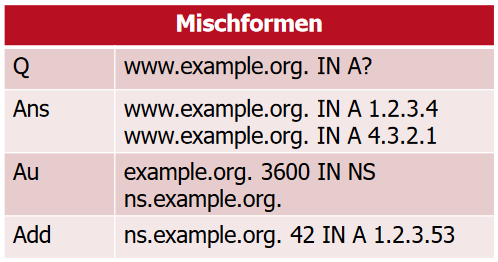
\includegraphics[scale=0.7]{Grafiken/DNS-Nachricht.png}
\caption{DNS Nachricht die die Antwort zur Frage liefert und auch noch die Adresse des für die Adresse zuständigen autoritativen Server mitteilt}
\end{figure} 

\begin{figure}[h!]
\centering
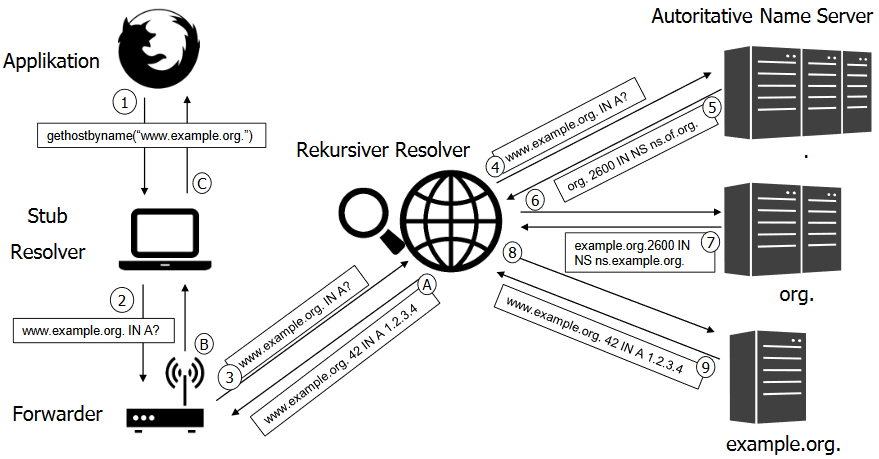
\includegraphics[scale=0.6]{Grafiken/DNS-Namensaufloesung.png}
\label{pic:DNS-Namensaufloesung}
\caption{Typischer Ablauf der Namensauflösung bei DNS}
\end{figure}

Die Namensauflösung ist \hyperref[pic:DNS-Namensaufloesung]{hier} dargestellt.\\
Dabei fragt der rekursive Resolver solange beim Root Name Server nach der Adresse und wird solange weiter verwiesen bis der autoritative Name Server ihm die Domain auflösen kann.\\
Hat der Forwarder die Antwort zu einer Domain bereits gecacht meldet er der Applikation direkt das gecachte Ergebnis zurück. Läuft die TTL ab fragt er erneut beim Resolver nach der Adresse.\\
Kennt der Resolver einen lower level autoritativen name server fragt er dort nach der Adresse und überspringt die höheren Ebenen.\\

Ein iterativer Resolver liefert nach der ersten Anfrage an einen autoritativen name server direkt eine Antwort zurück. Entweder die aufgelöste Adresse oder die Adresse des niedrigeren name servers, sodass der Forwarder erneut mit dieser Adresse nachfragen muss. 

\subsubsection{Angriffe auf DNS}

Beim \textbf{DNS Cache Poisoning} werden von einem Angreifer gefälschte Werte in einen DNS Cache eingetragen und untergraben damit die Authentizität der DNS Records im Cache.\\
Damit wird erreicht dass der Netzwerkverkehr zu bestimmten Domains auf die Server des Angreifers umgeleitet werden.\\

Möglichkeiten zur Impersonation von Diensten in der Ziel-Domain können durch folgende Möglichkeiten erreicht werden:
\begin{itemize}
\item Personifikation eines autoritativen Nameservers durch vergiftete Infrastrukturdaten
\item Personifizierung eines Dienstes in der Ziel-Domain
\item Subdomain Injection
\item Gezielte Manipulation beliebiger anderer Werte im Cache des Resolvers
\end{itemize}

Je nachdem wo das Cache Poisoning stattfindet sind entweder nur ein Client betroffen oder mehrere.\\

Beim Kashpureffs Angriff wurden gefälschte Records einer fremden Domain durch die Add section an den Resolver übermittelt, sodass sich dieser beim nächsten Auflösen an den anderen name server wendet.\\
Als Gegenmaßnahme wurde die ''Bailiwick-Regel'' eingeführt, wonach Resolver Records verwerfen müssen deren Namen sich nicht in einer Subdomain des Antwortservers befinden.\\
Zum Beispiel darf der name server (org.) nur Records aus der Zone .org., z.B. zu example.org. ausliefern.\\

Beim \textbf{Off-Path DNS Cache Poisoning} wird eine Anfrage zum Auflösen an den Resolver gesandt. Wenn dieser den Eintrag nicht gecacht hat sendet er die Anfrage an den passenden name server weiter. Der Angreifer sendet eine manipulierte Antwort im Namen des name servers (IP-Spoofing) an den Resolver. Sofern die Antwort des Angreifers vor der authentischen Antwort ankommt ist der Angriff geglückt.\\
Eine Herausforderung hierbei ist, dass der Angreifer die 16 Bit Transaction-ID im DNS-Header erraten muss. Wählt der Angreifer die Transaction-ID falsch wird die Antwort verworfen und die Antwort des name servers bleibt für die Dauer der TTL gespeichert.\\
Bei einem geglückten Angriff kann der Angreifer über den eingeschleusten bösartigen name server leicht weitere Werte einspeisen.\\
\begin{enumerate}
\item Sende Anfrage ''[nonce].vict.im IN A?'' an den Resolver
\item Sende Antwort nach obigem Format von der Opfer-IP-Adresse aus
	\begin{itemize}
	\item Möglichst viele Antworten mit unterschiedlichen Transaction-IDs (Schrotflintenprinzip)
	\end{itemize}
\item Bei Misserfolg, wiederhole bei (1)
\end{enumerate}
Als Gegenmaßnahme kann der UDP-Quellport (16 Bit) randomisiert werden, sodass sich mit der zufälligen Transaction-ID eine 32 Bit Zufallszahl ergibt. Aktuelle Bandbreiten sind hierfür nicht ausreichend. Die Gegenmaßnahme ist für MitM Angriffe unrelevant, da dieser die Nachrichten im Transit anpassen kann.\\

MitM Angriff auf rekursive Resolver im Internet ist mit \hyperref[txt:BGP-PrefixHijacking]{BGP Prefix Hijacking} realisierbar. MitM Angriff auf Stub-Resolver im lokalen Netz mit \hyperref[txt:spoofing]{ARP Cache Poisoning} oder im offenen WLAN möglich.\\

Eine weitere Gegenmaßnahme ist DNSSEC zu verweden, welches DNS Records signiert und die höheren name servern signieren die public keys ihrerer Kinder (Chain of trust).\\
Gewährt Integrität und Authentizität aber keine Vertraulichkeit. 
Allerdings werden die Antworten deutlich größer und erfordert mehr Aufwand beim Domain Betreiber.\\
Das Protokoll ist für 2nd Level Domains immer noch kaum verbreitet.\\

{\scriptsize
\begin{tabular}{|l|c|c|}
\hline
Record-Typ & Zweck & Wichtigste Werte in RData\\
\hline
DNSKEY & Bereitstellung des public key & Validierungsschlüssel, Signaturalgo\\
RRSIG & Bereitstellung der Signatur eines RRset & Typ und TTL des Sets, Signatur,...\\
DS & Verkettung zu Kind-Domain & Hashwert des Kindsschlüssel, Hashalgo, ...\\
NSEC/NSEC3 & Authentifizierung von Nicht-Exisitenz des Records & Hash nächsten Records\\
\hline
\end{tabular}
}

\begin{itemize}
\item DoT (DNS over TLS)
\item DHS (DNS over HTTPS)
\item Beide
	\begin{itemize}
	\item Sicherer Transport (Vertraulichkeit, Integrität, Authentifizierung)
	\item Sichern der Kommunikation zwischen Stub Resolver, Forwarder, Resolver
	\item Gewährleisten keine Authentizität der Daten
	\end{itemize}

\end{itemize}

Weitere Angriffe auf das DNS:
\begin{itemize}
\item Domain Hijacking
	\begin{itemize}
	\item Übernahme von Nutzerkonten bei Domain-Registraren
	\item Anfreifer kann dann legitimiert Werte im autoritativenn Server anpassen
	\end{itemize}
\item Flooding-Angriff gegen DNS-Server
	\begin{itemize}
	\item Üblicherweise durch Botnetz
	\item Durch zu viele Anfragen versagt der Dienst (DoS)
	\end{itemize}
\item Zensur des DNS
	\begin{itemize}
	\item Üblicherweise durch staatliche Stellen um Dienste zu sperren
	\item Betreiber von Resolvern (z.B. ISP) filtern Werte
	\item Kann durch das Verwenden von anderen Resolvern umgangen werden
	\end{itemize}
\end{itemize}

\subsubsection{Drittsystem Beeinflussung durch DNS}

Ein Endsystem wird durch fluten mit DNS Anfragen überlastet (DDoS).\\
Bei einem \textbf{DNS Amplification DDoS Angriff} senden Angreifersysteme mit gespoofter Opfer-IP-Adresse Anfragen an DNS Server. Die größeren Antwortpakete werden an das Opfer gesendet und überlastet dessen Systeme.\\
Als Gegenmaßnahme können die Kapazitätreserven an Netz und Systemen vergrößert werden und spezialisierte Weiterleitungsdienste mit starker Infrastruktur benutzt.\\
Der DNS Dienst kann die Antwortgröße minimieren um den Amplification-Faktor gering zu halten. DNSSEC wirkt hier kontraproduktiv.\\
Außerdem kann versucht werden Pakete mit gespoofter IP-Adresse im Ursprungsnetz zu filtern. Sicherheitsbehörden versuchen Botnetze stillzulegen.\\

Bei \textbf{DNS Tunneling} werden ausgespähte Informationen aus einem kompromittierten Netzwerk exfiltriert und Netzsperren und Firewalls umgangen. Außerdem können so Bots verdeckt mit ihrem Bot Master kommunizieren.\\
Hierzu setzt ein Angreifer einen autoritativen Server und Domain als Endpunkt auf, an den der Client Anfragen mit im Namen codierten Daten sendet. Die Resolver leiten dann unentdeckt diese Daten und die Antworten zwischen Angreifer und Client hin und her.\\
Mittels Firewalls bzw. IDS/IPS können mit statischer Anomaliedetektion solche auffälligen Anfragen gefiltert werden. Denn die angefragten Namenn sind häufig auffällig und es entsteht viel DNS-Verkehr zu einer oder wenigen Domains.\\

Mit dem \textbf{Sender Policy Framework} (SPF) wird das unautorisierte Versenden von Emails von einer Absender Domain (Email Spoofing) verhindert. Dafür spezifiziert der Domain Betreiber in seinen DNS Einträgen wer Emails senden darf. Der Empfänger holt sich diesen Record und lehnt die Email ab falls der Sender nicht autorisiert ist. Oftmals ineffektiv um nicht versehentlich legitime Emails zu blockieren.

Weitere Sicherheitsmechanismen sind:
\begin{itemize}
\item DKIM
	\begin{itemize}
	\item Verhindert Email Spoofing mit Signatur durch Absende-Server und Eintragen des public keys im DNS
	\end{itemize}
\item Domain Validation
	\begin{itemize}
	\item Automatisierte Ausstellung von TLS-Zertifikaten an Domain Inhaber, welche den public key an den Domain Namen binden
	\end{itemize}
\item DANE
	\begin{itemize}
	\item Erlaubt Nachweis der Echtheit von TLS Zertifikaten einer Domain durch DNS Einträge, benötigt DNSSEC
	\end{itemize}
\end{itemize}

\subsection{Border Gateway Protocol}

Datenpakete im lokalen Netz werden über Adresstabellen gerouted. Dabei speichert der routende Schwitch welche MAC an welchem Port anliegt. Beim ersten empfangen von Nachrichten an einem Port wird die MAC des Senders mit Port in die MAC Adress table gespeichert. Ist ein Empfänger nicht eingetragen, wird die Nachricht an alle Port ausgegeben (''fluten'').\\

Beim Routen mit IP-Adressen wird über den IP-Adressbereich (''Präfix'') geroutet, die Routingtabellen werden über das Border Gateway Protocol (BGP) gebildet.\\
Hierfür abstrahieren wir das Netzwerk in Knoten aus große autonomen Systemen (AS) was in sich gekapselte Netzwerke sind.\\
BGP kümmert sich nur um das Routing zwischen diesen Netzwerkknoten. Innerhalb der AS können verschiedene andere Protokolle zum Routen verwenden.\\
Jedes autonome System umfasst hierbei ein IP-Netz. Nachrichten zwischen ASs werden nach dem längsten Präfix gewählt und sonst nach der kürzesten Route. Beim Routen wird zum Beispiel der Pfad über den Knoten 1.1.1.0/24 zu 1.1.0.0/16 präferiert, selbst wenn dieser Pfad länger ist.\\

Beim BGP Sub-prefix hijacking leitet ein AS die Nachrichten über sein Netzwerk indem er den anderen ASs einen spezifischen Präfix mitteilt (''announcen''). Dadurch werden Daten über seinen Knoten geleitet, auch wenn es nicht der kürzeste Pfad ist. Dadurch sieht der Angreifer die komplette Kommunikation des Opfers. Beim same-prefix hijacking announced der AS den selben Präfix wie sein Opfer.\\
Der Sub-prefix Angriff betrifft prinzipiell alle Netze, beim same-prefix hijacking sind nur Netze mit kürzeren Routen zum Ziel betroffen.\\
Weiterhin können die umgeleiteten Daten nicht ans Ziel weitergeleitet werden, sondern das Netz simuliert die Webseite des Ziels und übernimmt die Rolle des Zieles.\\
BGP Hijacking ist relativ schwierig, da der Angreifer am ISP vorbei agieren muss um BGP-Speaker zu sein.\\
\label{txt:BGP-PrefixHijacking}

Gegenmaßnahmen:
\begin{itemize}
\item Regional Internet Registries (RIRs) betreiben Internet Routing Registries (IRRs), wo eingetragen wird wem welche Präfixe gehören
\item RPKIs können versichern dass dem Sender eines BGP announcements der Addressbereich gehört
\item IP-Raum von mindestens /24, d.h. 256 Adressen benötigt mit 20\$/Adresse 
\end{itemize}

\subsection{Sichere Verbindungen}

\begin{figure}[h!]
\centering
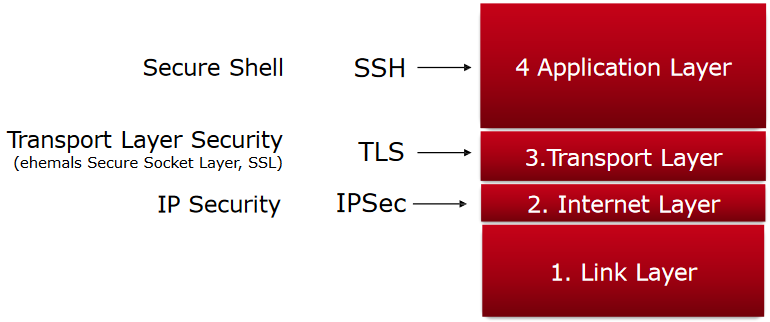
\includegraphics[scale=0.42]{Grafiken/Protokolle-nach-Ebene.png}
\caption{Sichere Verbindungsprotokolle nach TCP Ebene}
\end{figure}

\subsubsection{TLS}

TLS erfüllt die Schutzziele Authentizität des Kommunikationspartners, Vertraulichkeit der Daten (symmetrische Verschlüsselung) und Integrität der Daten (HMAC).\\
Sie bietet Replay Protection gegen das Wiedereinspielen alter Nachrichten, da Nonces verwendet werden.\\
(Perfect) forward secrecy schützt Daten auch wenn der private Schlüssel öffentlich wird.\\

\begin{figure}
\centering
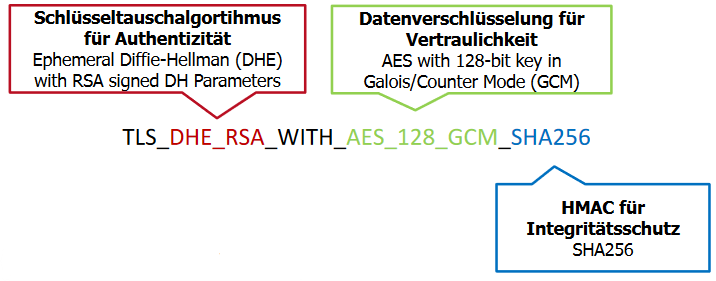
\includegraphics[scale=0.6]{Grafiken/Cipher-suites.png}
\caption{Cipher Suites spezifizieren die Parameter einer TLS-Session}
\end{figure}

Die TLS Verbindungsaufbau funktioniert wie folgt:
\setcounter{equation}{-1}
\begin{flalign}
CA \rightarrow Server:& \textrm{Zertifiziert public key des Servers}&&\\
Alice \rightarrow Server:& \textrm{Startet Verbindungsaufbau}\\
Alice \leftrightarrow Server:& \textrm{\hyperref[text:DiffieHellman]{Diffie-Hellman Schlüsselaustausch}}&&\\
Server \rightarrow Alice:& \textrm{Zertifikat + Signatur der DH-Parameter}&&\\
Alice \leftrightarrow Server:& \textrm{Sichere Kommunikation z.B. AES-GCM}&&
\end{flalign}

Bei (0) bekommt der Server von einer Certification Authority (CA) den Zusammenhang zwischen privaten key und Domainnamen zertifiziert. Die Zertifizierung funktioniert hierbei wie folgt:
\setcounter{equation}{0}
\begin{flalign}
Server:& \textrm{Generiert asymmetrisches Schlüsselpaar}&&\\
Server:& \textrm{Erstellt Zertifikatsrequest mit Name und public key}\\
Server:& \textrm{Signiert Request mit private key}&&\\
Server \rightarrow CA:& \textrm{Sendet signiertes Request}&&\\
CA \rightarrow Server:& \textrm{Prüft Identität und stellt Zertifikat aus}&&
\end{flalign}

In (2) kann sich Alice nicht sicher sein das sie mit dem Server kommuniziert (MitM). Erst in (3) authentifiziert sich der Server Alice gegenüber indem er seinen DH Parameter ($g^b$) signiert und mittels Zertifikat so Alice nachweist dass er kein Angreifer ist.\\
Eine Schwachstelle von TLS ist ein Fallback auf unverschlüsselte Kommunnikation, welche jedoch notwendig ist um Kompatibilität zu wahren.\\

TLS schützt Daten im Transit auf Anwendungsebene, d.h. jede Anwendung muss TLS selbst einbinden, es bietet aber keine Ende-zu-Ende-Verschlüsselung.

\subsubsection{IPSEC/VPN}

Ein Site-to-Site VPN ist eine verschlüsselte Verbindung zwischen dem Client und einem Server. Hierbei wird den Kommunikationspartnern des Clients simuliert, dass er sich innerhalb des selben privaten Netzes befindet.\\
Dafür wird das eigentliche IP-Paket verschlüsselt und mit einem neuen IP header versehen.\\
Das Anpassen des Headers wird hierbei vom Gateway realisiert und der Client weiß in der Regel nichts davon.\\

Im Transport Modus wo nur der Payload verschlüsselt ist bleiben die Adressen der Kommunikationspartner weiterhin sichtbar. Beim Tunnelmodus wo auch der Header verschlüsselt ist bleibten die Kommunikationspartner verborgen.\\

Beim Remote Access VPN wird der Rechner virtuell ins interne Netz integriert. Dabei weiß der Client dass er eine VPN Verbindung zu dem anderen Netz besitzt. Er besitzt seine normale IP-Adresse und eine IP-Adresse aus dem internen Netz.\\

\begin{tabular}{|c|c|c|}
\hline
& TLS & VPN\\
\hline
Start/Endpunkt & Client/Server & Client/Gateway\\
Verbindungssteuerung & Anwendung & Betriebssystem/Gateway\\
Verschlüsselte Daten & Anwendungsdaten & Alle Datenströme\\
Vertrauensanker & Zertifizierungsstellen & Manuelle Konfiguration\\
Protokolle & TLS, DTLS & IKE, IKEv2, IPSEC, OpenVPN,... \\
\hline
\end{tabular}

\subsubsection{Onion-Routing/TOR}
Pakete werden über das TOR Netzwerk versendet und dabei über eine variable Anzahl an Router geleitet bis sie das Ziel erreichen.\\
Dabei sieht jeder Router nur die Adresse von der sein Paket kam und wohin er es weiter leitet. Damit Sender und Empfänger keiner Partei bekannt wird, werden mindestens 3 Router benötigt.\\
TOR erschwert es Datenströme zuzuordnen, bietet aber keine perfekte Anonymität, da Pakete über korrelierende Paketgrößen zugeordnet werden (Metadaten).

\subsection{Public Key Infrastrukturen}

Wir unterscheiden drei Vertrauensmodelle:
\begin{itemize}
\item Direct Trust
	\begin{itemize}
		\item Kommunikationspartner tauschen öffentliche Schlüssel bzw. Zertifikate aus\\
		\item Schlüssel/Zertifikate müssen mit gespeicherten verglichen werden, sonst ist ein MitM Angriff möglich
		\item Nur relevant wenn sich Kommunikationspartner vorher kennen
	\end{itemize}
\item Hierarchical Trust
	\begin{itemize}
		\item Authentizität der Parteien durch Zertifikate von vertrauenswürdige Parteien (CAs)
		\item Schlüssel der CAs müssen separat übermittelt werden
		\item Zertifikatsstellen müssen selbst wieder vertrauenswürdig sein
	\end{itemize}
\item Web of Trust
	\begin{itemize}
		\item Vertreter ist PGP\\
		\item Introducer schafft für Dritte Vertrauen zu neuen Kommunikationspartnern
	\end{itemize}
\end{itemize}

Widerruf von Zertifikaten erfolgt mittels Zertifikatssperrlisten (CRL). Diese signierte Liste von gesperrten Zertifikaten einer CA sind in jedem Zertifikat verlinkt, sodass der Nutzer diese direkt überprüfen kann.\\
Mit dem Online Zertifikate Status Protokoll (OCSP) kann bei den CAs nachgefragt werden ob ein gegebenes Zertifikat noch gültig ist.\\
Da beides wenig genutzt wird, werden in der Regel einfach die Gültigkeitszeiträume von Zertifikaten verkürzt.\\

Siehe auch \ref{sec:Schlüsselverteilung}.

\end{document}